% !TeX root=../main.tex
\chapter{روش شناسی}

\section{مدل سیستم}

همان طور که در بخش های پیشین توضیح داده شد، ساختار سیستم $MLPM$ از دو بخش متحرک و ثابت تشکیل می شود که بخش مترحک حاوی آرایهی هالباخ بوده و بخش ثابت، سیم پیچ ها را شامل می شود. برای مدل سازی این سیستم، لازم است در نظر داشته باشیم که هدف نهایی از طراحی این سیستم کنترل دقیق موقعیت و جهت گیری بخش متحرک است. بنابراین، از این پس منظور از Plant سیستم پیشنهاد شده، تنها بخش متحرک آن است و سیم پیچ ها به عنوان عملگر شناخته می شوند که به صورت مجزا درباره ی آن توضیح داده خواهد شد.
در بخش اول از این قسمت، به توضیح مدل بخش متحرک سیستم خواهیم پرداخت.
\subsection{مدل سیستم متحرک}
در این سیستم، به دلیل وجود نداشتن نیروهای اتلافی از جمله اصطکاک و با صرف نظر از مقاومت هوا، می توان سیستم را به عنوان یک جسم ساده و با در نظر گرفتن جرم و ممان های اینرسی آن مدل کرد. بنابراین، روابط دینامیکی زیر برای این سیستم برقرار خواهد بود:
\begin{align}
	m \ddot{P_x} = F_x, \quad m \ddot{P_y} = F_y, \quad m \ddot{P_z} = F_z
\end{align}


\begin{align}
	I_{xx} \ddot{\alpha} = T_x, \quad I_{yy} \ddot{\beta} = T_y, \quad I_{zz} \ddot{\gamma} = T_z
\end{align}


در نتیجه، با محاسبه ی ماتریس های حالت برای این سیستم به صورت زیر خواهیم داشت:
\begin{equation}
	\dot{x} = A x + B u + g
\end{equation}
\begin{equation}
	y = C x + D u
\end{equation}
\begin{equation}
	A =
	\begin{bmatrix}
		0 & 1 & 0 & 0 & 0 & 0 & 0 & 0 & 0 & 0 & 0 & 0 \\
		0 & 0 & 0 & 0 & 0 & 0 & 0 & 0 & 0 & 0 & 0 & 0 \\
		0 & 0 & 0 & 1 & 0 & 0 & 0 & 0 & 0 & 0 & 0 & 0 \\
		0 & 0 & 0 & 0 & 0 & 0 & 0 & 0 & 0 & 0 & 0 & 0 \\
		0 & 0 & 0 & 0 & 0 & 1 & 0 & 0 & 0 & 0 & 0 & 0 \\
		0 & 0 & 0 & 0 & 0 & 0 & 0 & 0 & 0 & 0 & 0 & 0 \\
		0 & 0 & 0 & 0 & 0 & 0 & 0 & 1 & 0 & 0 & 0 & 0 \\
		0 & 0 & 0 & 0 & 0 & 0 & 0 & 0 & 0 & 0 & 0 & 0 \\
		0 & 0 & 0 & 0 & 0 & 0 & 0 & 0 & 0 & 1 & 0 & 0 \\
		0 & 0 & 0 & 0 & 0 & 0 & 0 & 0 & 0 & 0 & 0 & 0 \\
		0 & 0 & 0 & 0 & 0 & 0 & 0 & 0 & 0 & 0 & 0 & 1 \\
		0 & 0 & 0 & 0 & 0 & 0 & 0 & 0 & 0 & 0 & 0 & 0
	\end{bmatrix}
\end{equation}
\begin{equation}
	B =
	\begin{bmatrix}
		0 & 0 & 0 & 0 & 0 & 0 \\
		\frac{1}{m} & 0 & 0 & 0 & 0 & 0 \\
		0 & 0 & 0 & 0 & 0 & 0 \\
		0 & \frac{1}{m} & 0 & 0 & 0 & 0 \\
		0 & 0 & 0 & 0 & 0 & 0 \\
		0 & 0 & \frac{1}{m} & 0 & 0 & 0 \\
		0 & 0 & 0 & 0 & 0 & 0 \\
		0 & 0 & 0 & \frac{1}{I_{xx}} & 0 & 0 \\
		0 & 0 & 0 & 0 & 0 & 0 \\
		0 & 0 & 0 & 0 & \frac{1}{I_{yy}} & 0 \\
		0 & 0 & 0 & 0 & 0 & 0 \\
		0 & 0 & 0 & 0 & 0 & \frac{1}{I_{zz}}
	\end{bmatrix}
\end{equation}
\begin{equation}
	g =
	\begin{bmatrix}
		0 \\ 0 \\ 0 \\ 0 \\ 0 \\ -g \\ 0 \\ 0 \\ 0 \\ 0 \\ 0 \\ 0
	\end{bmatrix}
\end{equation}
\begin{equation}
	C = I_{12}, \quad
	D = 0_{12 \times 6}
\end{equation}


پارامتر های مورد استفاده در سیستم پیشنهاد شده دارای مقادیر زیر است:
\begin{align}
	m = 6.6 \text{ kg}, \quad g = 9.81 \text{m/s}^2
\end{align}
\begin{align}
	I_{xx} = 0.059 \text{ kg}\cdot\text{m}^2, \quad
	I_{yy} = 0.059 \text{ kg}\cdot\text{m}^2, \quad
	I_{zz} = 0.12 \text{ kg}\cdot\text{m}^2
\end{align}

\subsection{مدل سیستم ثابت}
عملگر سیستم که متشکل از 16 سیم پیچ که در آرایه ای 4 در 4 چیده شده اند می باشد، وظیفه ی اعمال نیرو و گشتاور تعیین شده توسط کنترلر را به متحرک بر عهده دارد. در صورتی که جریان الکتریکی گذرنده از هر سیم پیچ مشخص باشد، می توان نیرو و گشتاور برایند وارد بر متحرک را محاسبه کرد. البته به دلیل تعدد پارامتر ها و محدودیت های شبیه سازی، در این قسمت با استفاده از روش های تحلیلی، معادلاتی بر اساس داده های به دست آمده برای سیستم مورد نظر شناسایی شده است که در ادامه به شرح آنها خواهیم پرداخت.
\begin{enumerate}
	\item\textbf{ موقعیت سیم پیچ ها در دستگاه مختصات مرجع:}
	
	اولین مولفه ای که در این سیستم تعریف می شود، محل قرار گیری هر یک از سیم پیچ ها می باشد. در این مرحله، با در نظر گرفتن ابعاد سیم پیچ ها برابر با $\tau$ و تعداد سطر و ستون آرایه، محل قرار گیری مرکز هر یک مشخص می شود.  
	% Define Grid Parameters
	\begin{align}
		n_{\text{rows}} &= 4, \quad n_{\text{cols}} = 4
	\end{align}
	% Position Calculation for Each Coil
	\begin{align}
		x_{\text{center}, j} &= (j - 1) \cdot \tau - \frac{(n_{\text{cols}} - 1) \cdot \tau}{2}, \quad j = 1, \dots, n_{\text{cols}}
	\end{align}
	\begin{align}
		y_{\text{center}, i} &= (i - 1) \cdot \tau - \frac{(n_{\text{rows}} - 1) \cdot \tau}{2}, \quad i = 1, \dots, n_{\text{rows}}
	\end{align}
	\begin{align}
		z_{\text{center}} &= 0
	\end{align}
	در نهایت، موقعیت تمام سیم پیچ ها در سه راستای $x$، $y$ و $z$ در یک ماتریس ذخیره برای استفاده در مراحل بعد ذخیره می شود.
	% Final Position Matrix
	\begin{align}
		\mathbf{positions} =
		\begin{bmatrix}
			x_{\text{center}, 1}, y_{\text{center}, 1}, z_{\text{center}} \\
			x_{\text{center}, 2}, y_{\text{center}, 1}, z_{\text{center}} \\
			\vdots & \vdots & \vdots \\
			x_{\text{center}, n_{\text{cols}}}, y_{\text{center}, n_{\text{rows}}}, z_{\text{center}}
		\end{bmatrix}
	\end{align}
	
	\item\textbf{ موقعیت سیم پیچ ها در دستگاه مختصات متحرک:}
	
	برای محاسبه نیرو و گشتاور، نیاز به دانستن فاصله ی دقیق سیم پیچ مورد بررسی تا موقعیت متحرک وجود دارد. بنابراین، با اندازه گیری مختصات متحرک و استفاده از موقعیت های تعیین شده هر سیم پیچ، می توان بردار فاصله این دو را در دستگاه مختصات مبدا به دست آورد.
	% Corrected Position and Distance Calculations
	\begin{align}
		\mathbf{c^{m}} &= R 
		\begin{bmatrix}
			x_{\text{coil}} - x_m \\
			y_{\text{coil}} - y_m \\
			z_{\text{coil}} - z_m
		\end{bmatrix}
	\end{align}
	که در آن R ماتریس دوران تبدیل مختصات متحرک به دستگاه مختصات مبدا می باشد:
	\begin{align}
		R = R_z^T R_y^T R_x^T
	\end{align}
	% Rotation Matrices
	\begin{align}
		R_x =
		\begin{bmatrix}
			1 & 0 & 0 \\
			0 & \cos(\alpha_{\text{rotation}}) & -\sin(\alpha_{\text{rotation}}) \\
			0 & \sin(\alpha_{\text{rotation}}) & \cos(\alpha_{\text{rotation}})
		\end{bmatrix}
	\end{align}
	\begin{align}
		R_y =
		\begin{bmatrix}
			\cos(\beta_{\text{rotation}}) & 0 & \sin(\beta_{\text{rotation}}) \\
			0 & 1 & 0 \\
			-\sin(\beta_{\text{rotation}}) & 0 & \cos(\beta_{\text{rotation}})
		\end{bmatrix}
	\end{align}
	\begin{align}
		R_z =
		\begin{bmatrix}
			\cos(\gamma_{\text{rotation}}) & -\sin(\gamma_{\text{rotation}}) & 0 \\
			\sin(\gamma_{\text{rotation}}) & \cos(\gamma_{\text{rotation}}) & 0 \\
			0 & 0 & 1
		\end{bmatrix}
	\end{align}
	\item \textbf{محاسبه نیرو:}
	
	با در اختیار داشتن $c^{m}$، می توان بر اساس رابطه شناسایی شده به صورت زیر نیروی برایند ناشی از جریان های الکتریکی I را محاسبه کرد. 
	\begin{align}
		F_x &= K_x \cos(\eta_x) \sin(\eta_x) \\
		F_y &= K_y \sin(\eta_x) \cos(\eta_y) \\
		F_z &= K_z \sin(\eta_x) \sin(\eta_y)
	\end{align}
	که پارامتر های استفاده شده در این رابطه به صورت زیر است:
	
	\begin{align}
		\eta_x &= \frac{\pi}{\tau} \cdot c^{m}_1, \quad 
		\eta_y = \frac{\pi}{\tau} \cdot c^{m}_2
	\end{align}
	% Force Components
	\begin{align}
		K_x &= \alpha_x e^{\beta_k \cdot c^{m}_3}, \quad
		K_y = \alpha_y e^{\beta_k \cdot c^{m}_3}, \quad
		K_z = \alpha_z e^{\beta_k \cdot c^{m}_3}
	\end{align}
	\item \textbf{محاسبه گشتاور:}
	
	محاسبه ی گشتاور ناشی از هر سیم پیچ با استفاده از نیرو های محاسبه شده انجام می شود. با این تفاوت که علاوه بر آن، نیاز به محاسبه ی طول بازوی موثر نیز هست و با توجه به آنکه در این سیستم، بازوی فیزیکی وجود ندارد، لازم است طی محاسباتی این مقادیر محاسبه شوند. بنابراین خواهیم داشت:
	
	% Effective Radius Calculations
	\begin{align}
		r_{\text{eff},x1} &= c^{m}_1 - m_1 \tan(n c^{m}_1 + \frac{\pi}{2}) \\
		r_{\text{eff},x2} &= c^{m}_1 - m_2 \tan(n c^{m}_1 + \frac{\pi}{2}) \\
		r_{\text{eff},y1} &= c^{m}_2 - m_1 \tan(n c^{m}_1 + \frac{\pi}{2}) \\
		r_{\text{eff},y2} &= c^{m}_2 - m_2 \tan(n c^{m}_1 + \frac{\pi}{2}) \\
		r_{\text{eff},z1} &= -c^{m}_3 - \alpha_{rz} \\
		r_{\text{eff},z2} &= -c^{m}_3 - \alpha_{rz}
	\end{align}
	که در آن:
	\begin{align}
		m_1 &= \alpha_{m1} \cdot c^{m}_3 + \beta_{m1} \\
		m_2 &= \alpha_{m2} \cdot c^{m}_3 + \beta_{m2}
	\end{align}
	و
	\begin{align}
		n &= \frac{\pi}{\tau}
	\end{align}
	آنگاه، مقادیر گشتاور به صورت زیر محاسبه می شوند:
	% Torque Components
	\begin{align}
		T_x &= r_{\text{eff},y1} F_z - r_{\text{eff},z1} F_y \\
		T_y &= -r_{\text{eff},x1} F_z + r_{\text{eff},z2} F_x \\
		T_z &= r_{\text{eff},x2} F_y - r_{\text{eff},y2} F_x
	\end{align}
	
	\item \textbf{ماتریس $\Gamma$}
	
	در نهایت، پس از محاسبه ی روابط نیرو و گشتاور، می توان آنها را در یک ماتریس با نماد $\Gamma$ تعریف کرد که این ماتریس شامل تمام اطلاعات لازم برای محاسبه ی نیرو و گشتاور ناشی از گذر جریان در هر یک از سیم پیچ ها می باشد. این ماتریس به صورت زیر تعریف می شود:
	% Final Gamma Matrix
	\begin{align}
		\mathbf{\Gamma} =
		\begin{bmatrix}
			F_x \\ F_y \\ F_z \\ T_x \\ T_y \\ T_z
		\end{bmatrix}
	\end{align}
	و با در اختیار داشتن این ماتریس، مقدار پیچش\footnote{Wrench} ناشی از آن از ضرب ماتریسی زیر به دست می آید.
	\begin{equation}
		w_m_{net} = [w_m_1, w_m_2, \dots, w_m_n] [I_1, I_2, \dots, I_n]^T = \Gamma(\vec{c}_m) I,
	\end{equation}
	
	در صورتی که بخواهیم با در اختیار داشتن مقدار پیچش مورد نیاز، جریان های سیم پیچ ها را محاسبه کنیم، می توان از وارون ماتریس $\Gamma$ استفاده کرد. اما با توجه به ابعاد نامتقارن این ماتریس و برای مصرف حداقلی انرژی، برای محاسبه ی وارون از روش وارون مورس-پنروز استفاده می شود
\begin{equation}
	I = \Gamma^T (\Gamma \Gamma^T)^{-1} w_m_{net}.
\end{equation}
	
	پارامتر های استفاده شده برای این سیستم در جدول زیر نمایش داده شده اند:
	\begin{table}[h]
		\centering
		\begin{tabular}{|c|c|}
			\hline
			\textbf{Parameter} & \textbf{Value} \\
			\hline
			$\tau$ & $0.0508$ \\
			$\beta_k$ & $-87.14$ \\
			$\alpha_x$ & $3.9021$ \\
			$\alpha_y$ & $3.9021$ \\
			$\alpha_z$ & $5.5209$ \\
			$\alpha_{m1}$ & $-0.0715$ \\
			$\alpha_{m2}$ & $-0.1046$ \\
			$\beta_{m1}$ & $-0.123$ \\
			$\beta_{m2}$ & $-0.0203$ \\
			$\alpha_{rz}$ & $-0.0146$ \\
			$n_{\text{rows}}$ & $4$ \\
			$n_{\text{cols}}$ & $4$ \\
			$dT$ & $0.01$ \\
			$Mass$ & $6.6$ \\
			\hline
		\end{tabular}
		\caption{جدول پارامترها}
		\label{tab:parameters}
	\end{table}
	
\end{enumerate}
\subsection{پیاده سازی محاسبات ماتریس حالت}
برای پیاده سازی ماتریس حالت، از کد متلب زیر استفاده شده است:
 \begin{latin}
 	\begin{minted}[frame=lines, linenos, breaklines]{matlab}
function [xdot, y] = System_SS_Model(u, x)
% Parameters
m = 6.6;            % Mass (kg)
g = 9.81;           % Gravitational acceleration (m/s^2)

% Moment of Inertia
Ixx = 0.059;        % Moment of inertia around x-axis
Iyy = 0.059;        % Moment of inertia around y-axis
Izz = 0.12;         % Moment of inertia around z-axis

% State vector x = [Px, Vx, Py, Vy, Pz, Vz, α, ω_x, β, ω_y, γ, ω_z]
% Input vector u = [Fx, Fy, Fz, Tx, Ty, Tz]

% State-Space Matrix (continuous time)
A = zeros(12, 12);
% Position-velocity couplings
A(1,2) = 1;  % Px dot = Vx
A(3,4) = 1;  % Py dot = Vy
A(5,6) = 1;  % Pz dot = Vz
A(7,8) = 1;  % α dot = ω_x
A(9,10) = 1; % β dot = ω_y
A(11,12) = 1;% γ dot = ω_z

% Input Matrix (continuous time)
B = zeros(12, 6);
% Force to acceleration conversion
B(2,1) = 1/m;    % Fx -> ax
B(4,2) = 1/m;    % Fy -> ay
B(6,3) = 1/m;    % Fz -> az
% Torque to angular acceleration conversion
B(8,4) = 1/Ixx;  % Tx -> α_ddot
B(10,5) = 1/Iyy; % Ty -> β_ddot
B(12,6) = 1/Izz; % Tz -> γ_ddot

% Gravitational effect (constant acceleration in z direction)
gravity = zeros(12,1);
gravity(6) = -g;  % Acceleration in z direction

% State derivative (continuous time)
xdot = A * x + B * u + gravity;

% Output equation (we'll output all states)
y = x;
end
 	\end{minted}
 \end{latin}
 برای اعتبارسنجی سیستم ارائه شده در این بخش، با اعمال ورودی صفر به سیستم، رفتار آن را مشاهده می کنیم. انتظار می رود تا جسم مطابق روابط سقوط آزاد، در راستای z پایین برود. همچنین، مقادیر محاسبه شده برای سرعت و موقعیت جسم در این راستا طبق روابط زیر به دست می آیند و انتظار  می رود تا در پاسخ سیستم نیزز مشاهده شود.
 \begin{equation}
 	P_z(t) = P_{z0} + V_{z0} t - \frac{1}{2} g t^2
 \end{equation}
 با در نظر گرفتن سرعت و موقعیت اولیه ی صفر خواهیم داشت:
 \begin{equation}
 	P_z(1) = -\frac{1}{2} (9.81) (1)^2 = -4.905 \text{ m}
 \end{equation}
 همچنین در محاسبات سرعت خواهیم داشت:
 \begin{equation}
 	V_z(t) = V_{z0} - g t
 \end{equation}
 \begin{equation}
 	V_z(1) = - (9.81) (1) = -9.81 \text{ m/s}
 \end{equation}
 با بررسی شبیه سازی پاسخ سیستم خواهیم داشت:
 \begin{figure}[H]
 	\centering
 	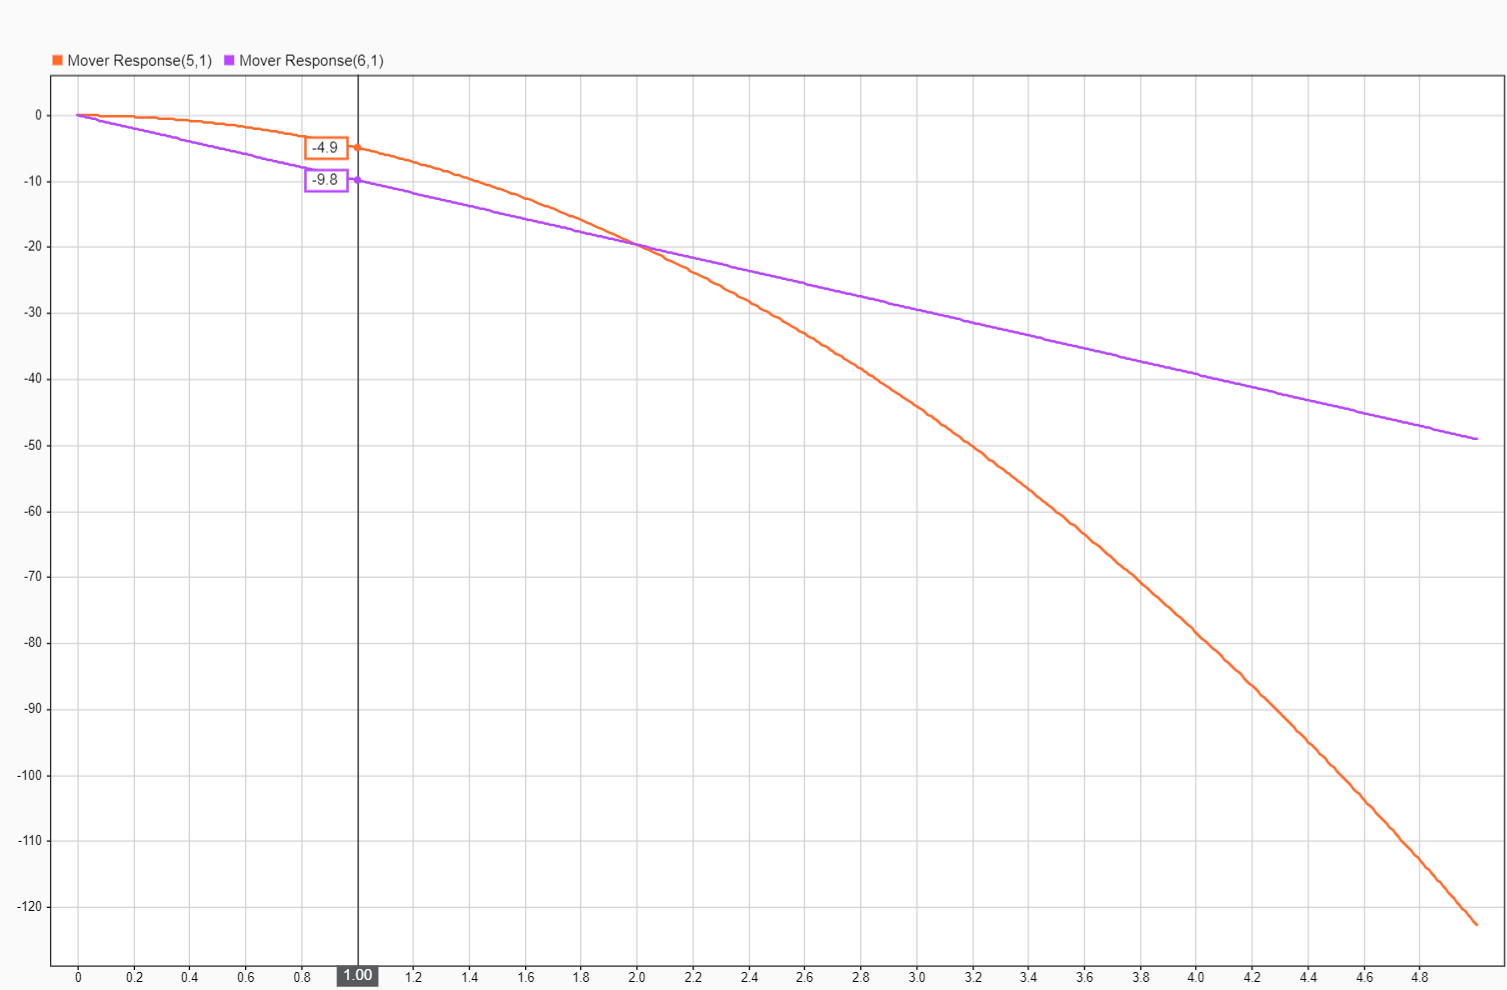
\includegraphics[width=1\linewidth]{../img/Mover_fall_verification}
 	\caption{اعتبارسنجی مدل سیستم متحرک}
 	\label{fig:moverfallverification}
 \end{figure}
 
\subsection{پیاده سازی محاسبات $\Gamma$}
برای اجرای محاسبات توضیح داده شده در بخش قبل، با استفاده از کد متلب زیر، تابعی برای محاسبه ی ماتریس $\Gamma$ ایجاد می شود:

\begin{latin}
	\begin{minted}[frame=lines, linenos, breaklines]{matlab}
	% Define symbolic variables
	syms Cxm Cym Czm tau beta_k alpha_x alpha_y alpha_z pi
	syms x_m y_m z_m alpha_rotation_m beta_rotation_m gamma_rotation_m % Added rotation angles
	syms alpha_m1 alpha_m2 beta_m1 beta_m2 alpha_rz
	
	% Step 1: Generate fixed positions of coils in global coordinates
	tau = sym('tau');
	
	n_rows = 4;
	n_cols = 4;
	positions = sym(zeros(n_rows * n_cols, 3));
	row_idx = 0;
	for i = 1:n_rows
	for j = 1:n_cols
	row_idx = row_idx + 1;
	x_center = (j - 1) * tau - ((n_cols - 1) * tau / 2);
	y_center = (i - 1) * tau - ((n_rows - 1) * tau / 2);
	z_center = 0;
	positions(row_idx, :) = [x_center, y_center, z_center];
	end
	end
	
	positions_func = matlabFunction(positions, 'File', 'generateCoilPositions1', ...
	'Vars', tau);   
	
	% Step 2: Define rotation matrices
	Rx = [1, 0, 0;
	0, cos(alpha_rotation_m), -sin(alpha_rotation_m);
	0, sin(alpha_rotation_m), cos(alpha_rotation_m)];
	
	Ry = [cos(beta_rotation_m), 0, sin(beta_rotation_m);
	0, 1, 0;
	-sin(beta_rotation_m), 0, cos(beta_rotation_m)];
	
	Rz = [cos(gamma_rotation_m), -sin(gamma_rotation_m), 0;
	sin(gamma_rotation_m), cos(gamma_rotation_m), 0;
	0, 0, 1];
	
	% Calculate complete rotation matrix (transpose of RxRyRz)
	R = transpose(Rz) * transpose(Ry) * transpose(Rx);
	
	% Calculate Gamma matrix with force and torque
	num_coils = size(positions, 1);
	Gamma = sym(zeros(6, num_coils));
	n = pi / tau;
	
	for i = 1:num_coils
	% Coil position in global coordinates
	coil_pos_g = positions(i, :);
	
	% Calculate position difference and apply rotation
	pos_diff = [coil_pos_g(1) - x_m;
	coil_pos_g(2) - y_m;
	coil_pos_g(3) - z_m];
	
	% Apply rotation matrix to get cm
	cm = R * pos_diff;
	
	% Calculate eta_x and eta_y for this coil
	eta_x = pi * cm(1) / tau;
	eta_y = pi * cm(2) / tau;
	
	% Calculate Kx, Ky, and Kz for this coil
	Kx = alpha_x * exp(beta_k * cm(3));
	Ky = alpha_y * exp(beta_k * cm(3));
	Kz = alpha_z * exp(beta_k * cm(3));
	
	% Calculate force terms
	Fx_term = Kx * cos(eta_x) * sin(eta_y);
	Fy_term = Ky * sin(eta_x) * cos(eta_y);
	Fz_term = Kz * sin(eta_x) * sin(eta_y);
	
	% Calculate m1 and m2
	m1 = alpha_m1 * cm(3) + beta_m1;
	m2 = alpha_m2 * cm(3) + beta_m2;
	
	% Calculate effective radius terms
	r_eff_x1 = cm(1) - m1 * tan(n * cm(1) + pi/2);
	r_eff_x2 = cm(1) - m2 * tan(n * cm(1) + pi/2);
	r_eff_y1 = cm(2) - m1 * tan(n * cm(1) + pi/2);
	r_eff_y2 = cm(2) - m2 * tan(n * cm(1) + pi/2);
	r_eff_z1 = -cm(3) - alpha_rz;
	r_eff_z2 = -cm(3) - alpha_rz;
	
	% Calculate torque terms
	T_x_term = r_eff_y1 * Fz_term - r_eff_z1 * Fy_term;
	T_y_term = -r_eff_x1 * Fz_term + r_eff_z2 * Fx_term;
	T_z_term = r_eff_x2 * Fy_term - r_eff_y2 * Fx_term;
	
	% Combine force and torque terms in gamma_i
	gamma_i = [Fx_term; Fy_term; Fz_term; T_x_term; T_y_term; T_z_term];
	
	% Add gamma_i as a column in the Gamma matrix
	Gamma(:, i) = gamma_i;
	end
	
	% Create MATLAB function with updated variables including rotation angles
	matlabFunction(Gamma, 'File', 'computeFullGammawithTorqueR4', 'Vars', {x_m, y_m, z_m, ...
		alpha_rotation_m, beta_rotation_m, gamma_rotation_m, tau, beta_k, ...
		alpha_x, alpha_y, alpha_z, alpha_m1, alpha_m2, beta_m1, beta_m2, alpha_rz, pi});
	\end{minted}
\end{latin}

برای اعتبار سنجی سیستم در این بخش با در نظر گرفتن ماتریس های گاما و وارون آن، انتظار آن می رود که ورودی های وارد شده به ماتریس وارون گاما که در سیستم عملیاتی توسط کنترلر تولید می شوند، پس از خروج از ماتریس گاما دقیقا مقادیری برابر با ورودی داشته باشند. با بررسی این مورد در سیستم زیر خواهیم داشت:
% TODO: \usepackage{graphicx} required
\begin{figure}[H]
	\centering
	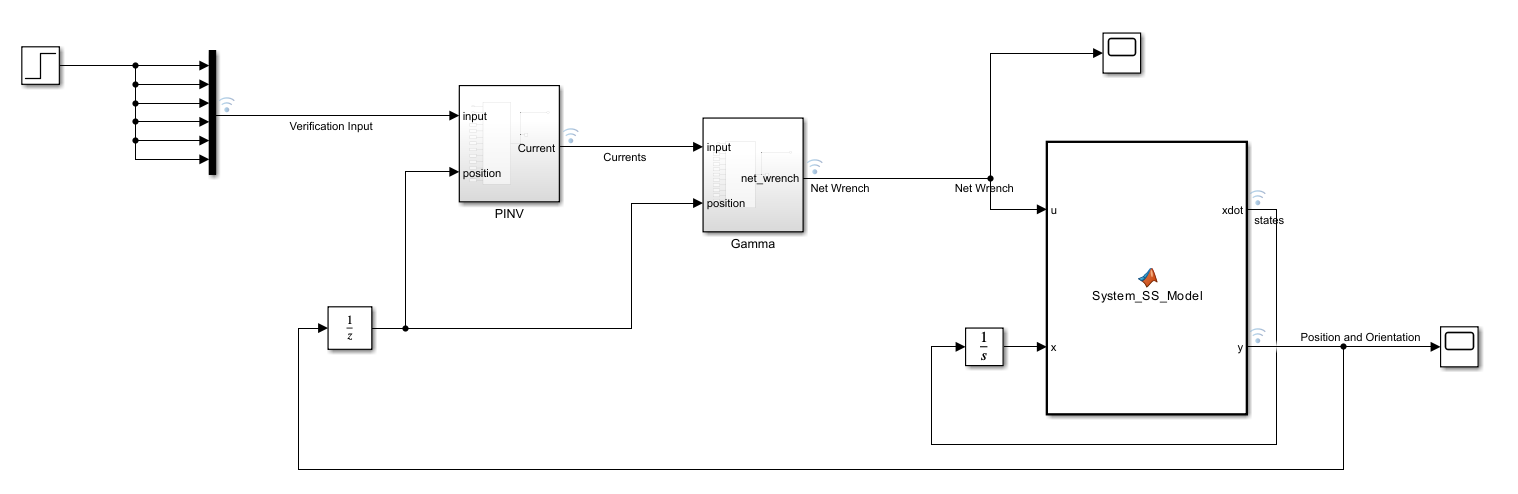
\includegraphics[width=1\linewidth]{../img/Gamma_Verification_diagram}
	\caption{دیاگرام سیستم اعتبارسنجی سیم پیچ ها}
	\label{fig:gammaverificationdiagram}
\end{figure}
% TODO: \usepackage{graphicx} required
\begin{figure}[H]
	\centering
	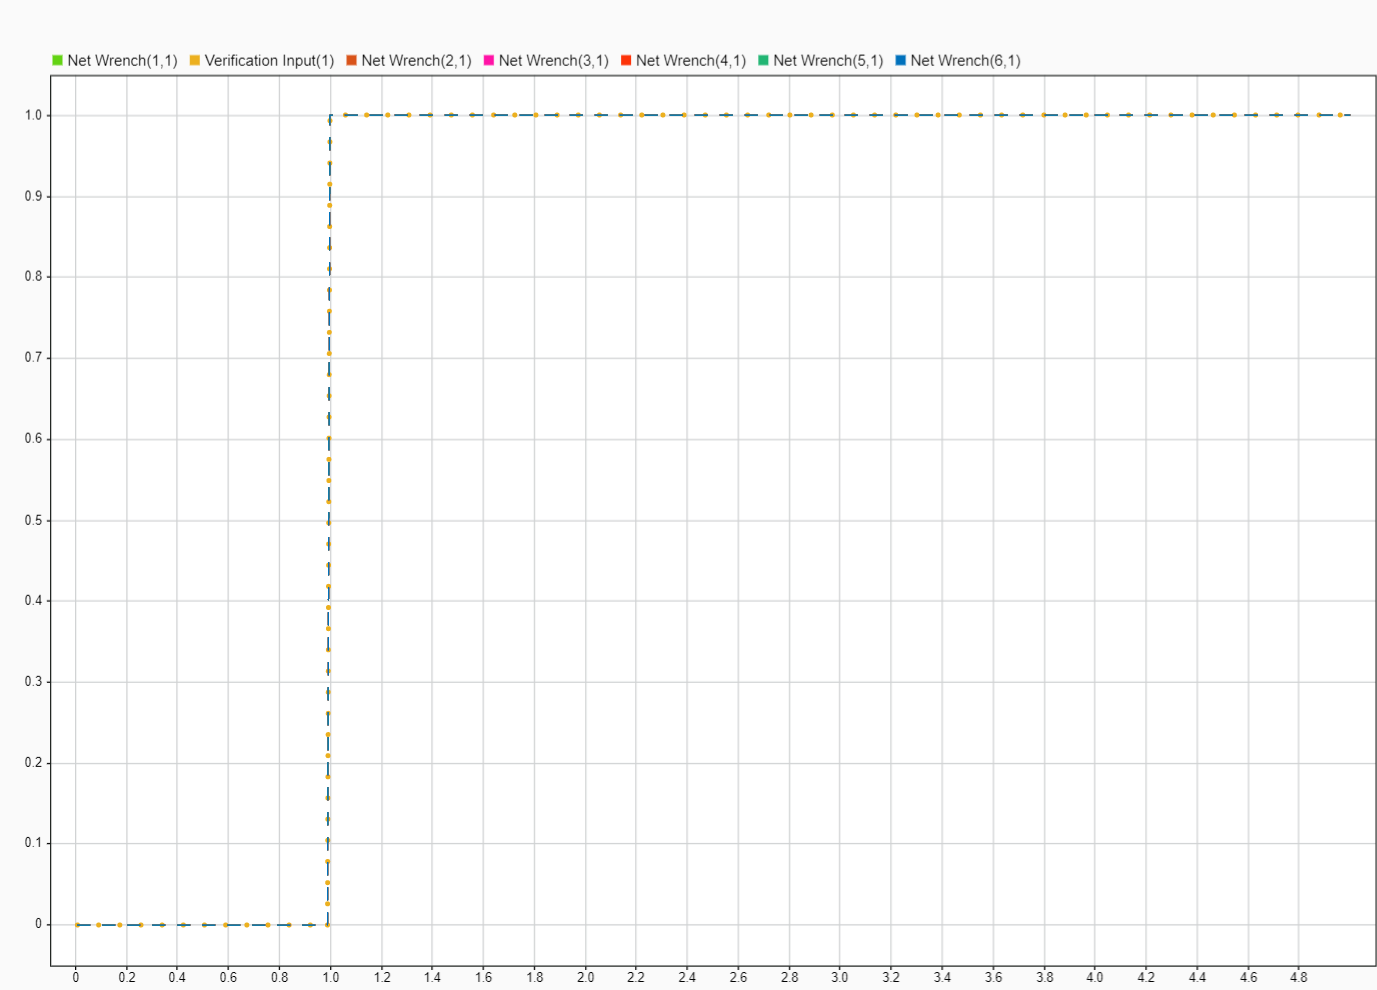
\includegraphics[width=1\linewidth]{../img/Gamma_Verification}
	\caption{اعتبار سنجی سیستم سیم پیچ ها}
	\label{fig:gammaverification}
\end{figure}

\section{طراحی کنترلر}
با مشخص شدن مدل سیستم، می توان آن را در محیط سیمولینک پیاده سازی کرد. برای این منظور، با قرار دادن بلوک های مناسب و اتصال آنها، این سیستم به صورت زیر مشخص می شود.
\begin{figure}[H]
	\centering
	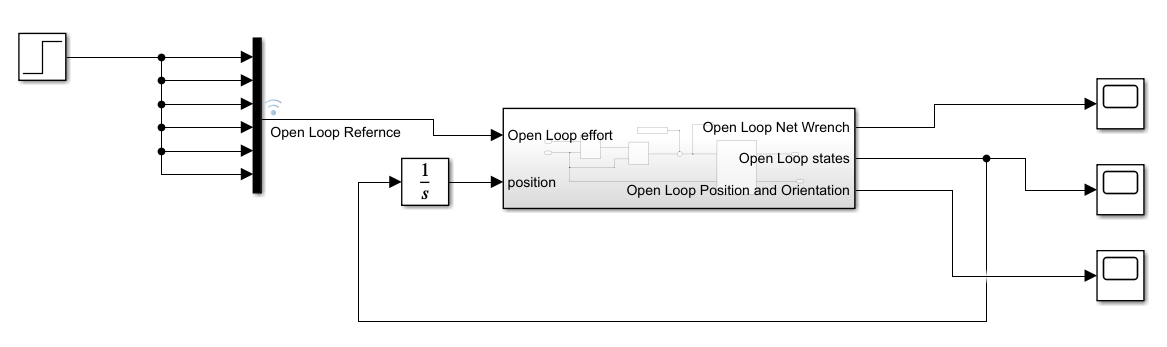
\includegraphics[width=1\linewidth]{../img/Plant}
	\caption{مدل سیستم}
	\label{fig:plant}
\end{figure}
همانطور که در این تصویر نمایش داده شده است، زیر سیستم های مربوط به متحرک، محاسبه ی ماتریس گاما و وارون آن و معادلات دینامیکی متحرک سیستم طراحی شده اند. علاوه بر این، شایان ذکر است که با در نظر گرفتن نیروی گرانش وارد بر متحرک، مقدار این نیرو به صورت اغتشاش و مجزا از ساختار کنترلی طبق رابطه ی زیر محاسبه شده و در راستای محور z به سیستم وارد شده است. 

در ادامه ی این فصل، به بررسی پاسخ های این سیستم و طراحی کنترلر های مناسب برای آن خواهیم پرداخت.

\subsection{پاسخ سیستم حلقه باز}
با اعمال ورودی پله واحد برای موقعیت ها و جهت گیری ها، پاسخ سیستم به صورت زیر به دست می آید:
\begin{figure}[H]
	\centering
	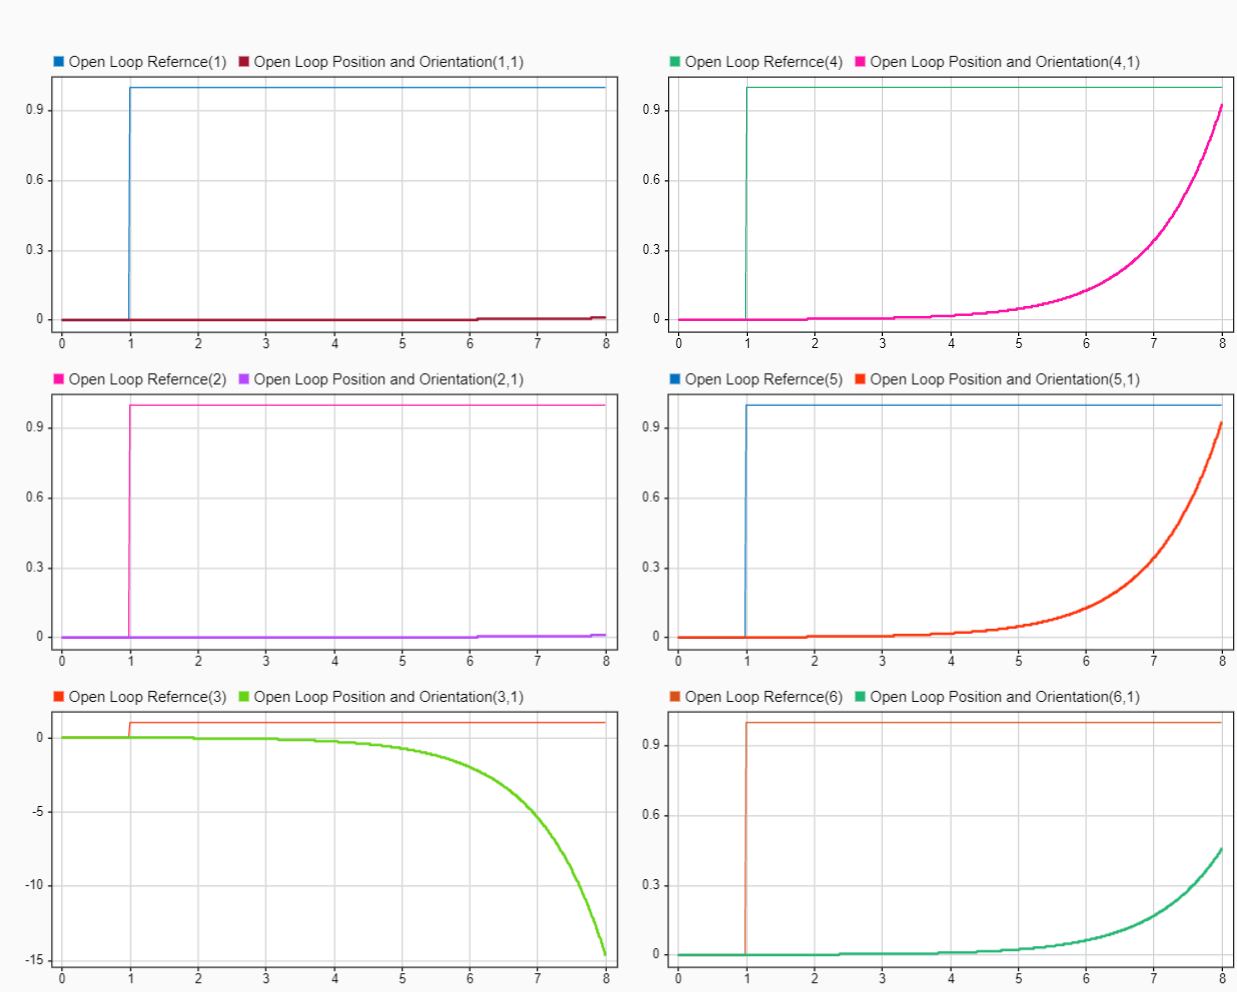
\includegraphics[width=1\linewidth]{../img/openloop_response}
	\caption{پاسخ حلقه باز سیستم}
	\label{fig:openloopresponse}
\end{figure}
مشاهده می شود که در کنترل موقعیت و جهتگیری، سیستم به صورت ذاتی پایدار نیست و نیاز به پیاده سازی کنترلر دارد. علاوه بر این، خصوصا در راستای محور z برای جلوگیری از فرو افتادن متحرک، نیاز به کنترل بیشتری است.
بنابراین، در گام بعد یک کنترلر PID برای این سیستم طراحی می شود و پاسخ آن بررسی می شود.
\subsection{پیاده سازی کنترلر $PID$}
با تشکیل حلقه ی فیدبک و قرار دادن کنترلر PID در سیستم، ساختار آن به صورت زیر تشکیل می شود.
% TODO: \usepackage{graphicx} required
\begin{figure}[H]
	\centering
	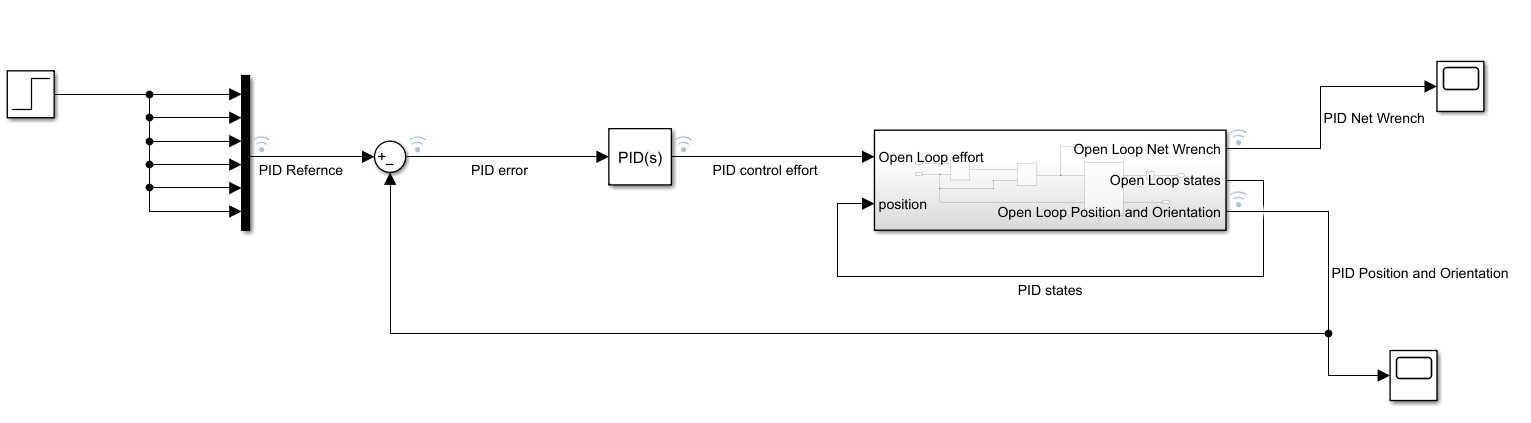
\includegraphics[width=1\linewidth]{../img/PID_diagram}
	\caption{دیاگرام سیستم با کنترلر $PID$}
	\label{fig:piddiagram}
\end{figure}
با تنظیم ضرایب PID چند متغیره برای هر معیار، در نهایت پاسخ پله ی سیستم در کنار تلاش کنترلی آن به صورت زیر به دست می آید:
% TODO: \usepackage{graphicx} required
\begin{figure}[H]
	\centering
	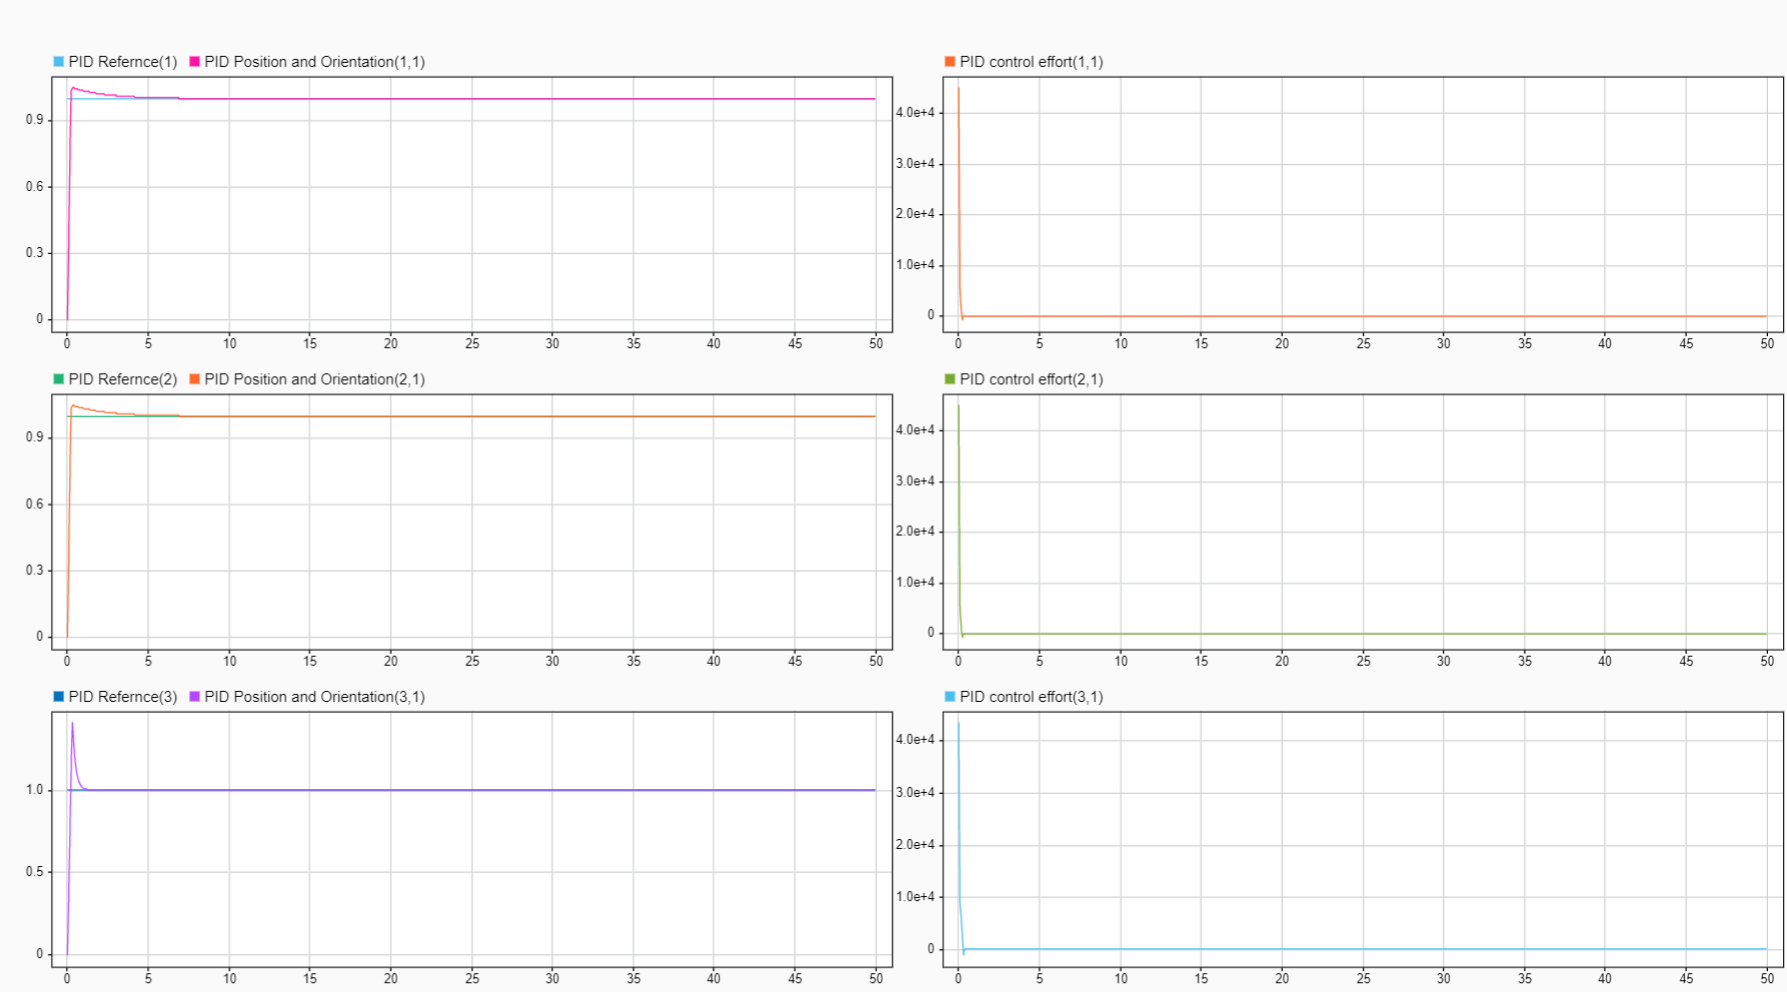
\includegraphics[width=0.7\textheight]{../img/PID_Response2_position}
	\caption{پاسخ پله و تلاش کنترلی برای کنترل موقعیت}
	\label{fig:pidresponse_position}
\end{figure}
در اینجا نیز مشاهده می شود که پاسخ به دست آمده در راستای محور Z همچنان تفاوت هایی با سایر محور ها دارد که ناشی از اعمال جاذبه به ان است. اما با قرار دادن بهره های کنترلی بالاتر برای این محور، زمان رسیدن به پاسخ مناسب تری به دست آورده است.
\begin{figure}[H]
	\centering
	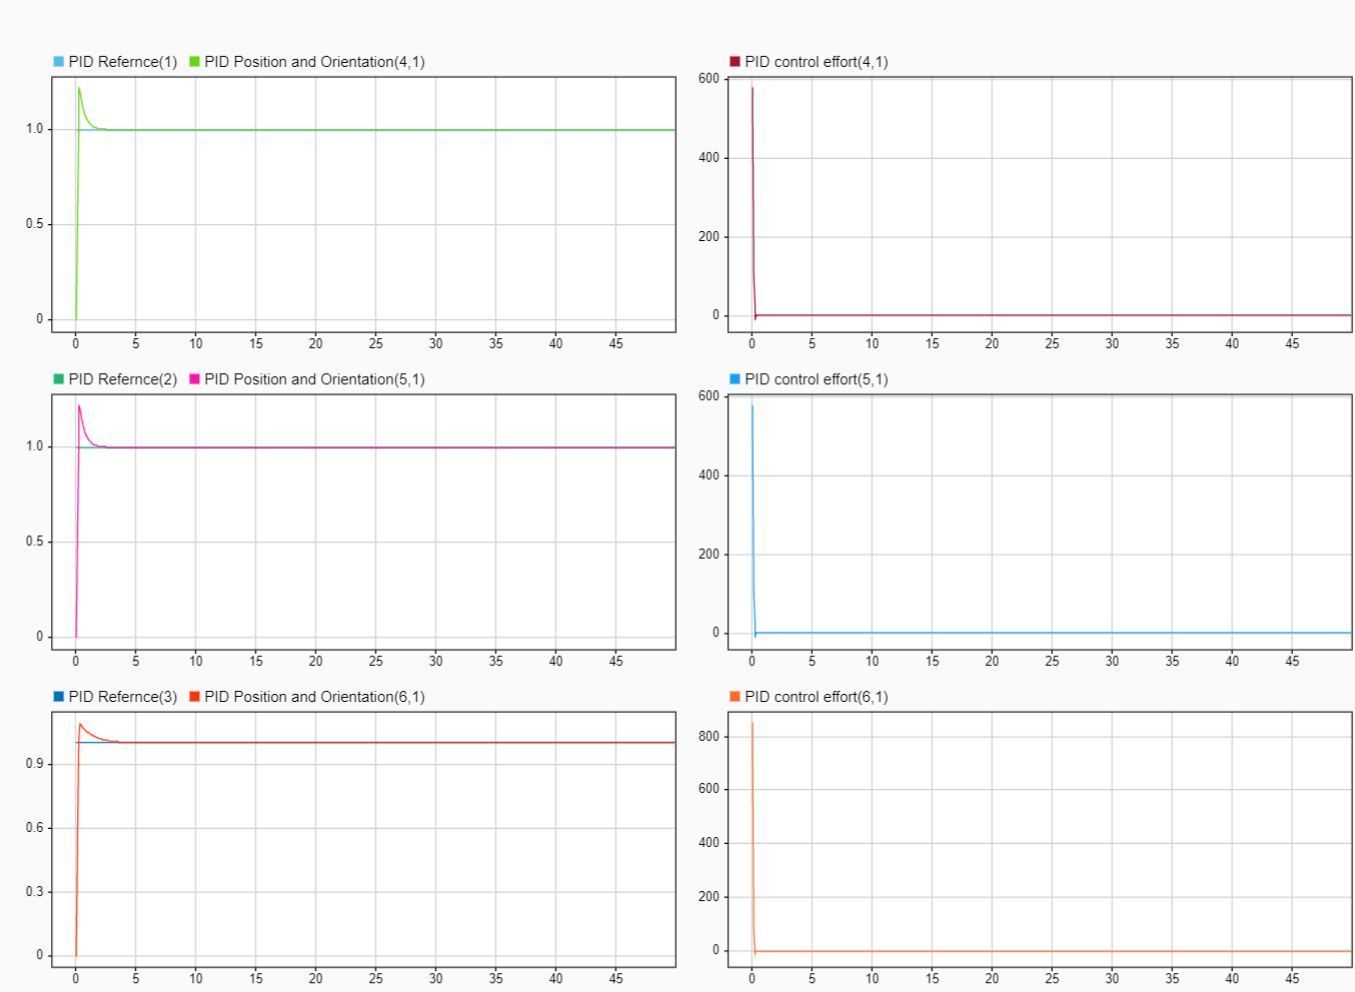
\includegraphics[width=0.7\textheight]{../img/PID_Response2_orinetation}
	\caption{پاسخ پله و تلاش کنترلی برای کنترل جهت گیری}
	\label{fig:pidresponse_orientation}
\end{figure}
ضرایب PID به کار رفته در این سیستم در جدول زیر نمایش داده شده اند.
\begin{table}[H]
	\centering
	\begin{tabular}{c|c|c|c}
		\hline
		\textbf{Axis} & \textbf{P Gain} & \textbf{I Gain} & \textbf{D Gain} \\
		\hline
		x & $10000$ & $4800$ & $350$ \\
		y & $10000$ & $4800$ & $350$ \\
		z & $13000$ & $30000$ & $325$ \\
		$\alpha$ & $180$ & $400$ & $4$ \\
		$\beta$ & $180$ & $400$ & $4$ \\
		$\gamma$ & $200$ & $180$ & $6.5$ \\
		\hline
	\end{tabular}
	\caption{ضرایب کنترلر PID}
	\label{tab:pid_gains}
\end{table}
\[
N = 100
\]

\subsection{پیاده سازی کنترلر $Linear MPC$}
در بخش بعد، با جایگذاری یک کنترلر MPC به جای PID و اتصال سیگنال های مربوط به آن، ساختار سیستم به صورت زیر به دست می آید.
\begin{figure}[H]
	\centering
	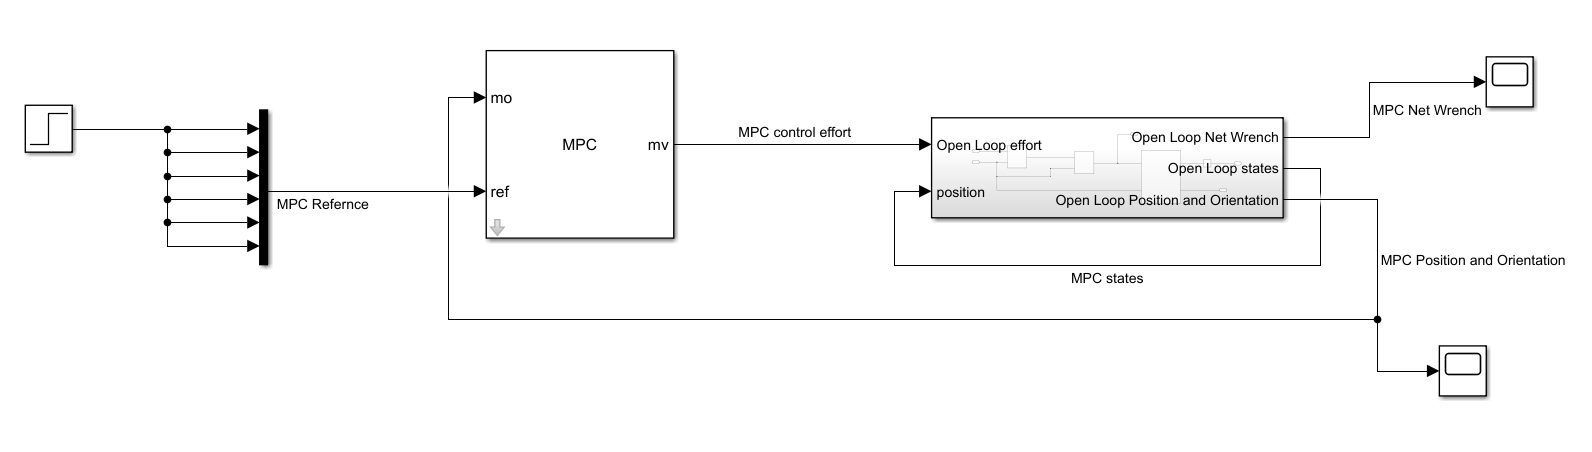
\includegraphics[width=0.9\linewidth]{../img/LMPC_diagram}
	\caption{دیاگرام کنترلر $Linear MPC$}
	\label{fig:lmpcdiagram}
\end{figure}

در ادامه به طراحی کنترلر MPC می پردازیم. برای این کار، در ابتدا تنظیمات تعداد ورودی و خروجی کنترلر و افق پیش بین آن را تنظیم می کنیم.
\begin{figure}[H]
	\centering
	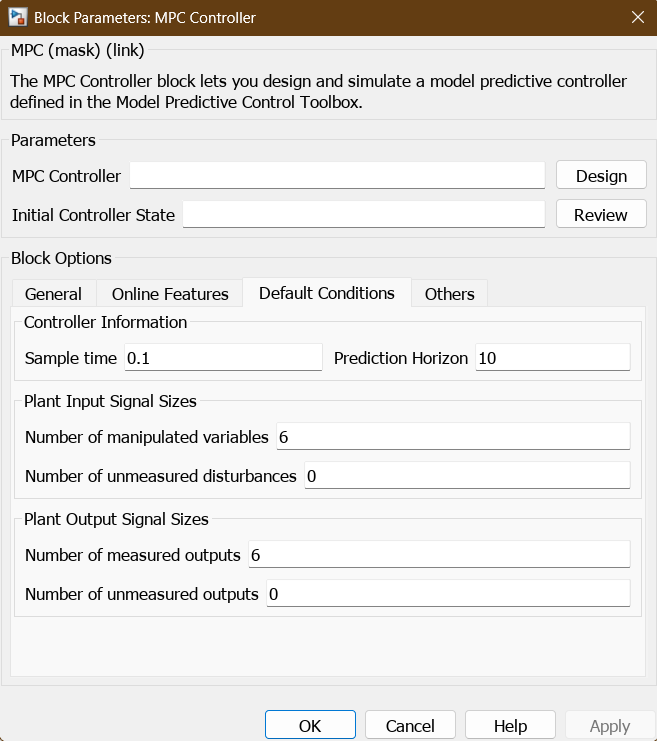
\includegraphics[width=0.7\linewidth]{../img/LMPC_Config}
	\caption{تنظیمات $MPC$}
	\label{fig:lmpcconfig}
\end{figure}

در ادامه با استفاده از جعبه ابزار کنترلر پیش بین، کنترلر را طراحی می کنیم. با تنظیم افق پیش بین بر مقدار 100 و افق کنترلی بر مقدار 30 مطابق تصویر زیر می توانیم پاسخ های سیستم کنترل شده را مشاهده کنیم.
\begin{figure}[H]
	\centering
	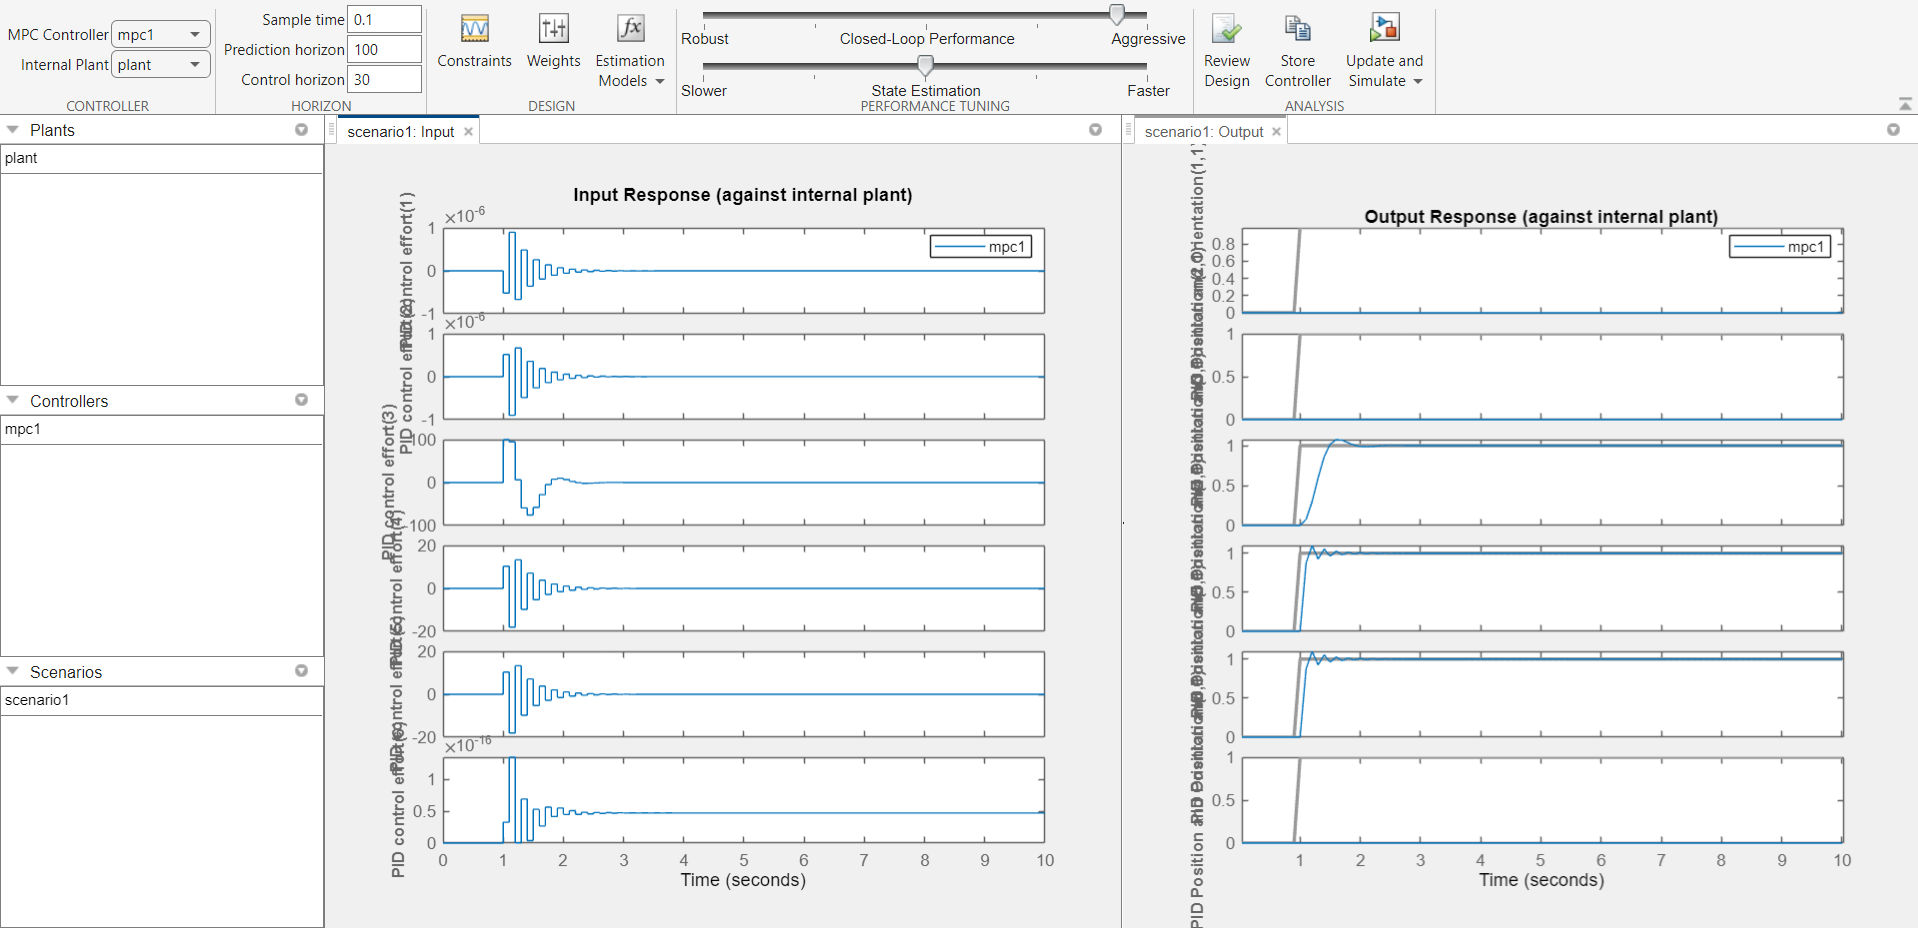
\includegraphics[width=1\linewidth]{../img/LMPC_Setup}
	\caption{طراحی کنترلر $MPC$}
	\label{fig:lmpcsetup}
\end{figure}

همانطور که در تصویر بالا مشاهده می شود، این کنترلر موقعیت عمودی و جهت گیری حول محور های افقی سیستم را می تواند به خوبی کنترل کند، اما برای سه حالت دیگر قادر به ایجاد فرمان های کنترلی مناسب نیست. 
با در نظر داشتن این مورد برای این کنترلر، پاسخ آن را مشاهده می کنیم.
\begin{figure}[H]
	\centering
	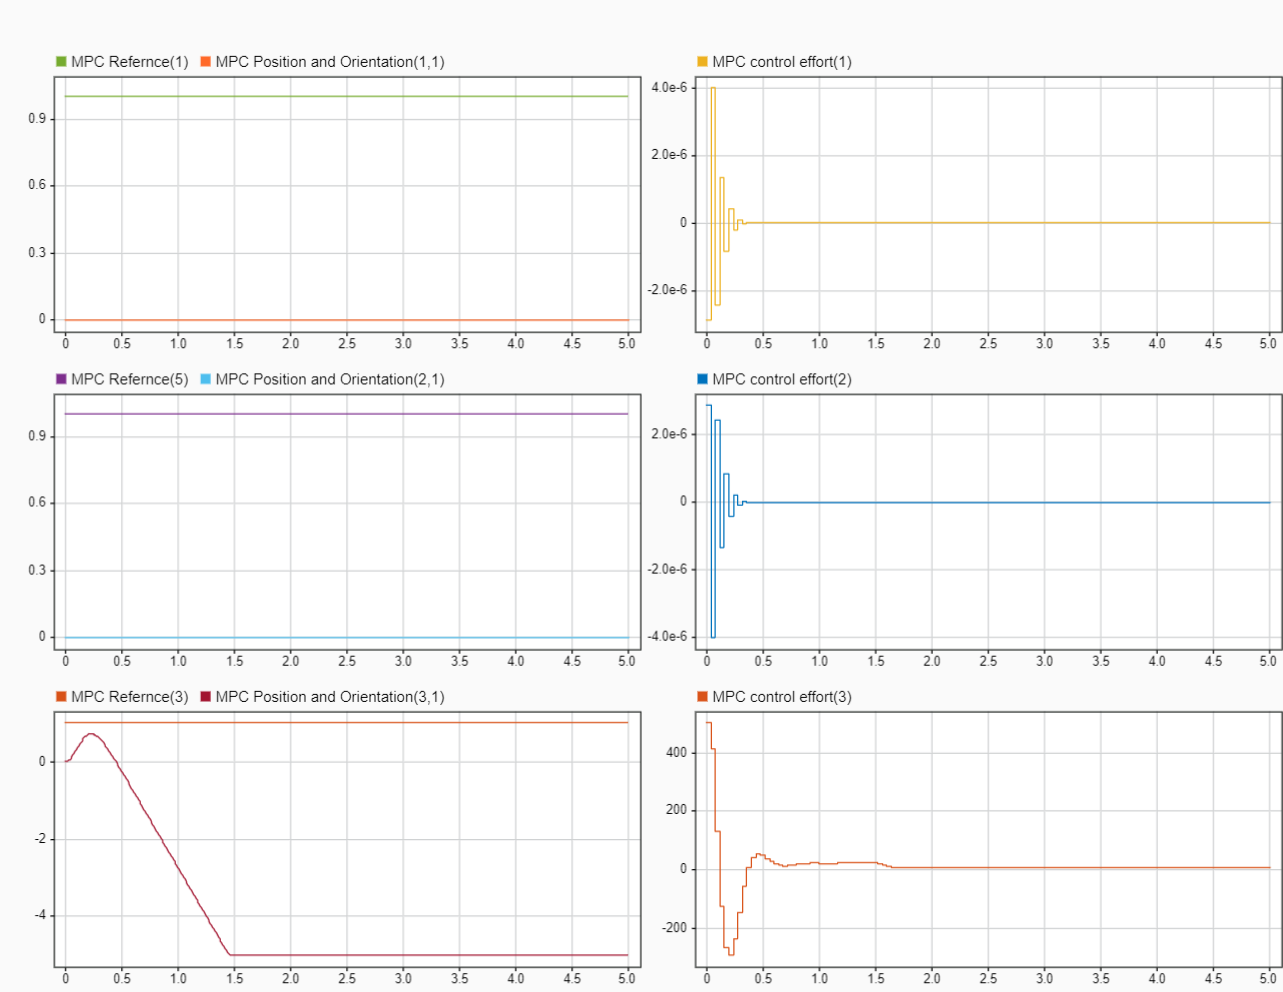
\includegraphics[width=1\linewidth]{../img/LMPC_Response_Position}
	\caption{پاسخ کنترلر $LMPC$ برای کنترل موقعیت}
	\label{fig:lmpcresponseposition}
\end{figure}
\begin{figure}[H]
	\centering
	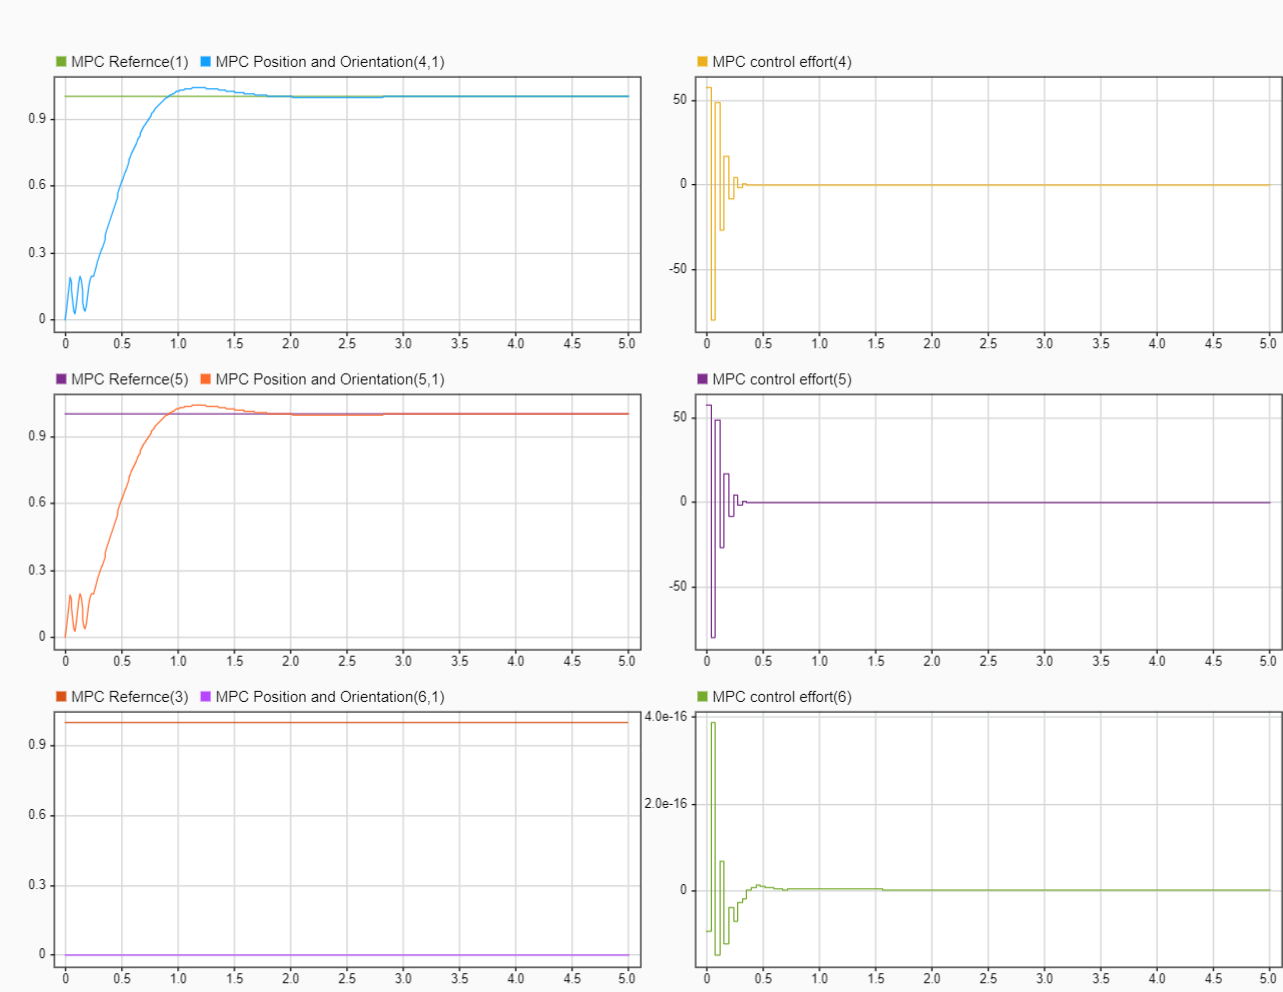
\includegraphics[width=1\linewidth]{../img/LMPC_Response_Orientation}
	\caption{پاسخ کنترلر $LMPC$ برای کنترل جهت گیری}
	\label{fig:lmpcresponseorientation}
\end{figure}

همان طور که در تصاویر بالا مشاهده می شود، این کنترلر به جز در تعیین جهت گیری و زاویه ی سیستم حول محور های دوران x و y، قادر به کنترل سیستم نیست. علاوه بر این، علی رغم پاسخ های مشاهده شده در تنظیم سیستم برای کنترل موقعیت در راستای z، علی رغم وجود تلاش کنترلی به دلیل ماهیت غیرخطی سیستم شناوری مغناطیسی در ارتفاع های مختلف، قادر به کنترل سیستم نمی باشد. در اینجا لازم به یادآوری است که معادلات دینامیکی شناسایی شده برای سیستم در ارتفاع 15 میلی متری تعیین شده است و بنابراین تنها با در نظر گرفتن مدل سیستم، نمی توان موقعیت ارتفاع آن را کنترل کرد.

\subsection{پیاده سازی کنترلر $Tube MPC$}

با توجه به عملکرد کنترلر LMPC و PID، در این بخش به طراحی کنترلر $Tube MPC$ خواهیک پرداخت. با در نظر داشتن عملکرد کنترلر LMPC برای موقعیت ها و جهت گیری ها، می توان نتیجه گرفت که استفاده از کنترلر PID برای کنترل مد هایی که MPC قادر به کنترل آنها نبود می تواند راهکار مناسبی باشد. علاوه بر این، برای کاهش زمان پاسخ در مد های کنترل شده نیز، استفاده از PID کمک کننده است. 
بنابراین، ساختار کنترلی این سیستم به صورت زیر تشکیل می شود.
\begin{figure}[H]
	\centering
	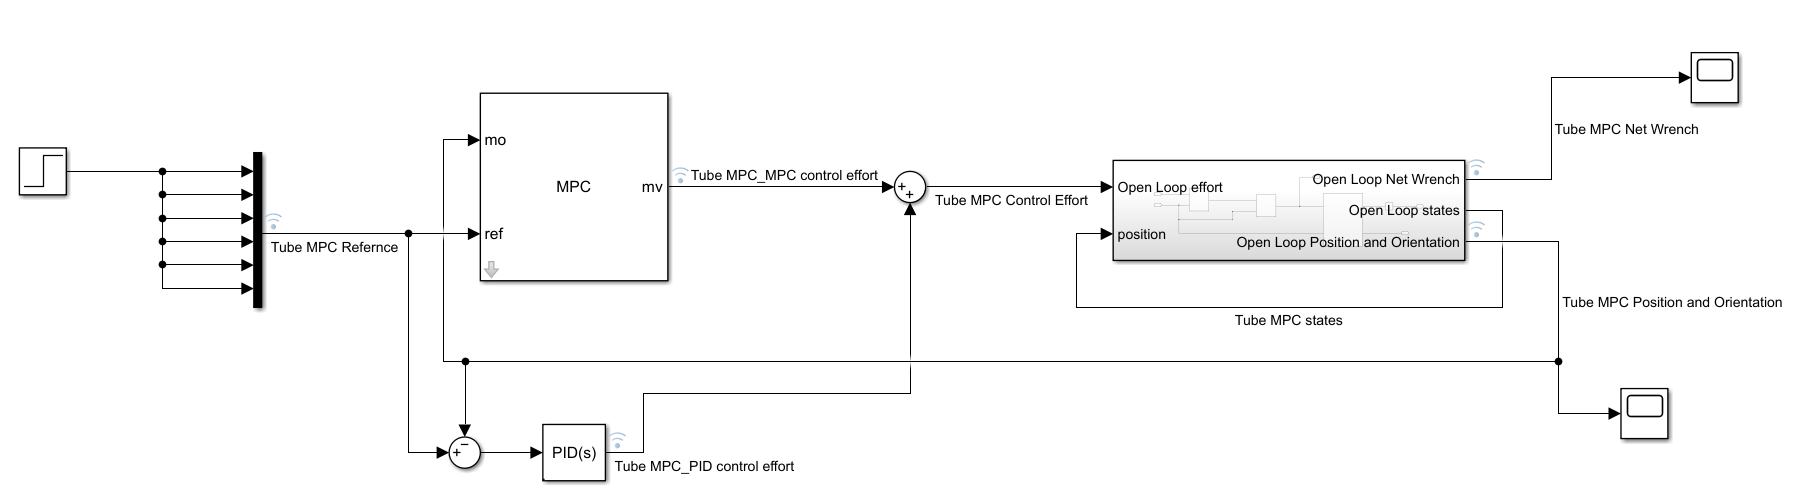
\includegraphics[width=1\linewidth]{../img/TMPC_Diagram}
	\caption{دیاگرام کنترلر TMPC}
	\label{fig:tmpcdiagram}
\end{figure}

پاسخ سیستم به ورودی پله به صورت زیر خواهد بود.
\begin{figure}[H]
	\centering
	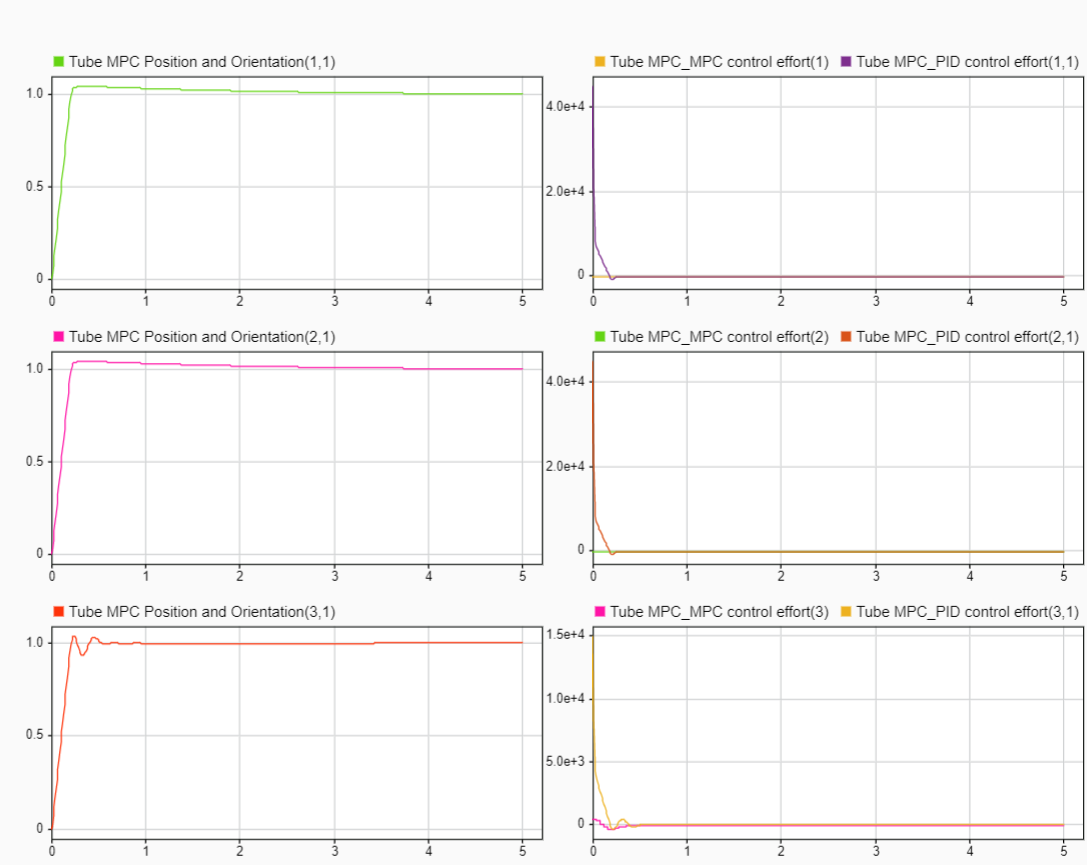
\includegraphics[width=1\linewidth]{../img/TMPC_Response_Position}
	\caption{پاسخ کنترلر TMPC به ورودی پله برای کنترل موقعیت}
	\label{fig:tmpcresponseposition}
\end{figure}
\begin{figure}[H]
	\centering
	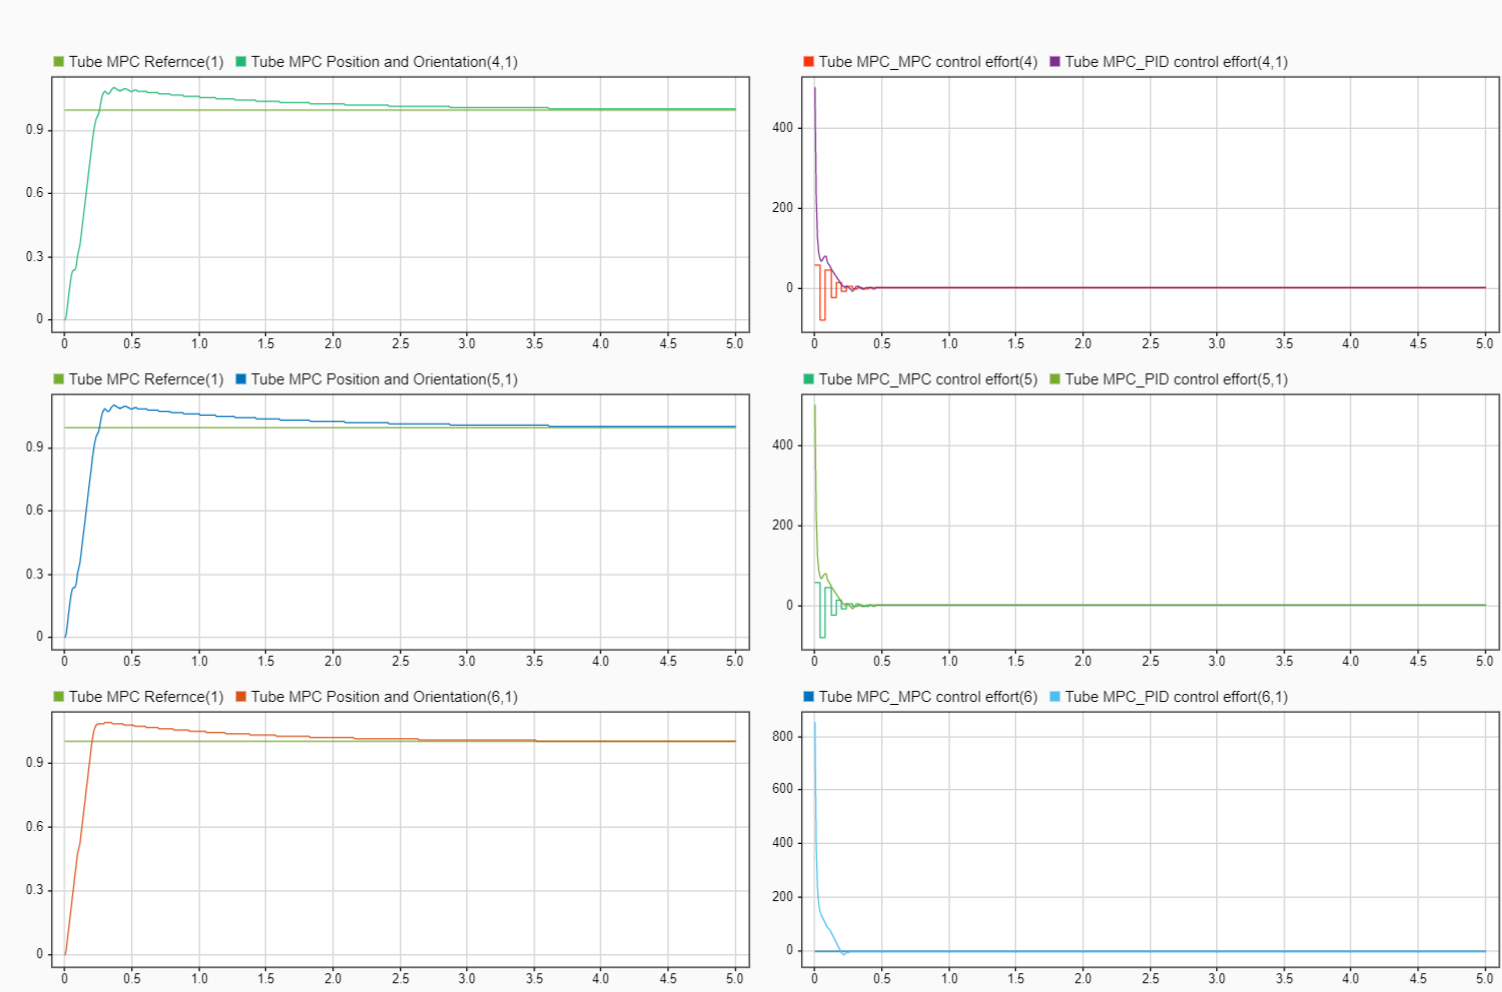
\includegraphics[width=1\linewidth]{../img/TMPC_Response_Orientation}
	\caption{پاسخ کنترلر TMPC به ورودی پله برای کنترل جهت گیری}
	\label{fig:tmpcresponseorientation}
\end{figure}

ضرایب کنترلر PID مورد استفاده در این بخش به صورت زیر است:
\begin{table}[H]
	\centering
	\begin{tabular}{c|c|c|c}
		\hline
		\textbf{Axis} & \textbf{P Gain} & \textbf{I Gain} & \textbf{D Gain} \\
		\hline
		x & $10000$ & $4800$ & $350$ \\
		y & $10000$ & $4800$ & $350$ \\
		z & $5000$ & $500$ & $100$ \\
		$\alpha$ & $100$ & $80$ & $4$ \\
		$\beta$ & $100$ & $80$ & $4$ \\
		$\gamma$ & $200$ & $180$ & $6.5$ \\
		\hline
	\end{tabular}
	\caption{ضرایب کنترلر PID در TMPC}
	\label{tab:Tube_pid_gains}
\end{table}


\section{مقایسه نتایج}
با بررسی های انجام شده بر سیستم MLPM و اعتبارسنجی مدل آن که به تفصیل در بخش اول از این فصل انجام شد، می توان عملکرد کنترلر های مختلف را بر روی این سیستم بررسی و مقایسه کرد. در بخش قبل، ساختار کنترلر های PID، LMPC و TMPC شرح داده شده و پاسخ پله ی آنها به ورودی پله مشاهده شد. 
اما برای بررسی دقیق تر، در این بخش مقادیر نویز و اغتشاش نیز به سیستم اعمال شده و پاسخ هر یک از حالت های مورد اندازه گیری سیستم را به وسیله کنترلر های مختلف بررسی می کنیم.
در گام اول، مقدار در زمان 3 ثانیه به هر یک از حالت های سیستم اعمال می شود.
\begin{figure}[H]
	\centering
	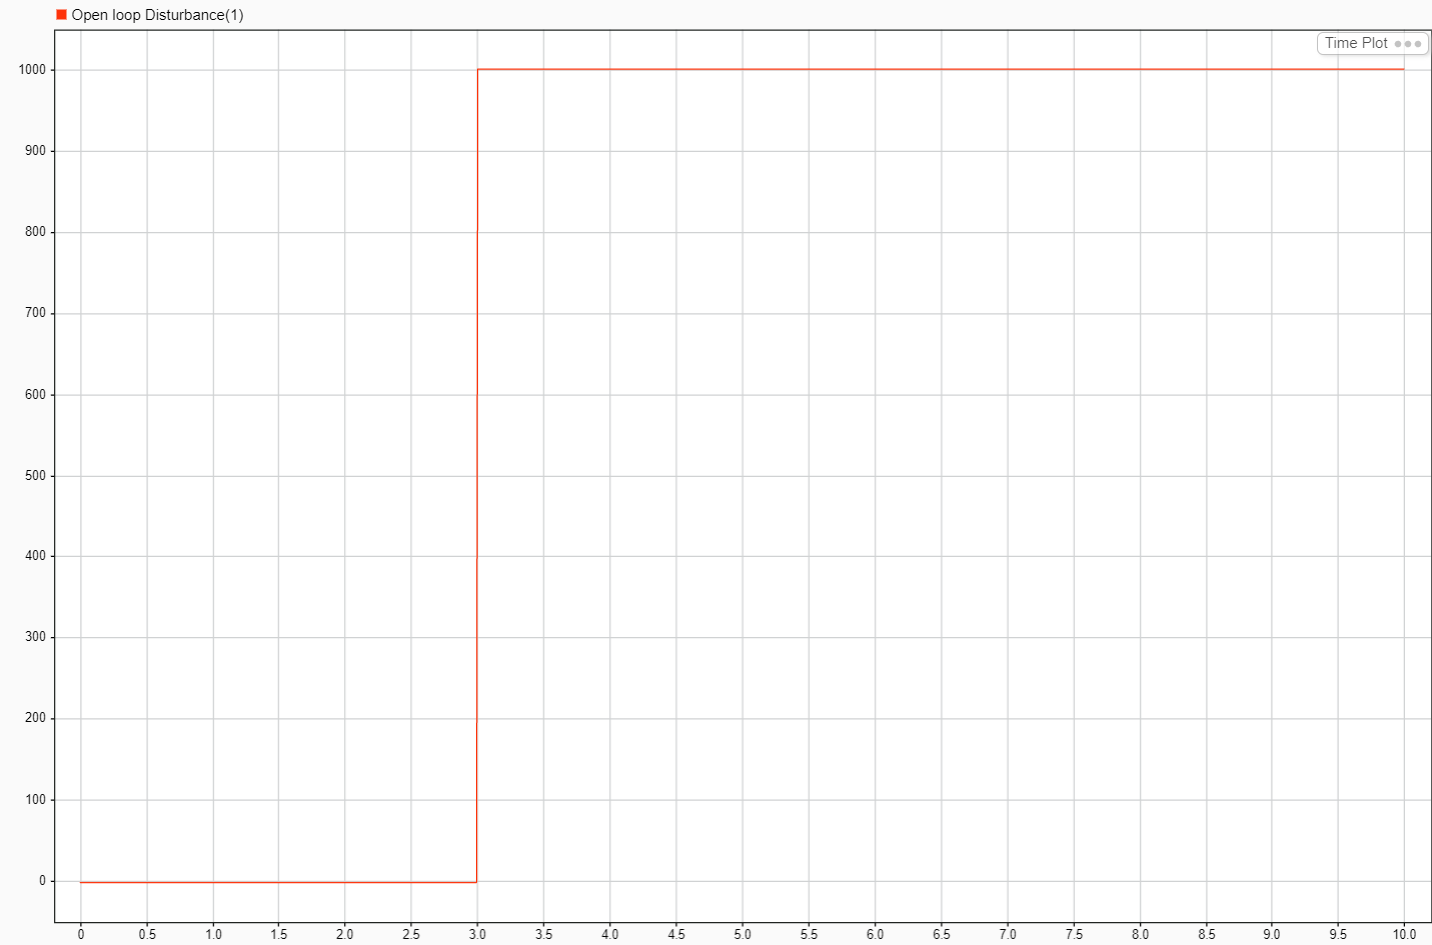
\includegraphics[width=1\linewidth]{../img/Disturbance}
	\caption{نمودار اغتشاش}
	\label{fig:disturbance}
\end{figure}

این اغتشاش به طور مستقیم به متحرک وارد می شود. بنابراین، مدل سیستم به صورت زیر تغییر پیدا می کند.
\begin{figure}[H]
	\centering
	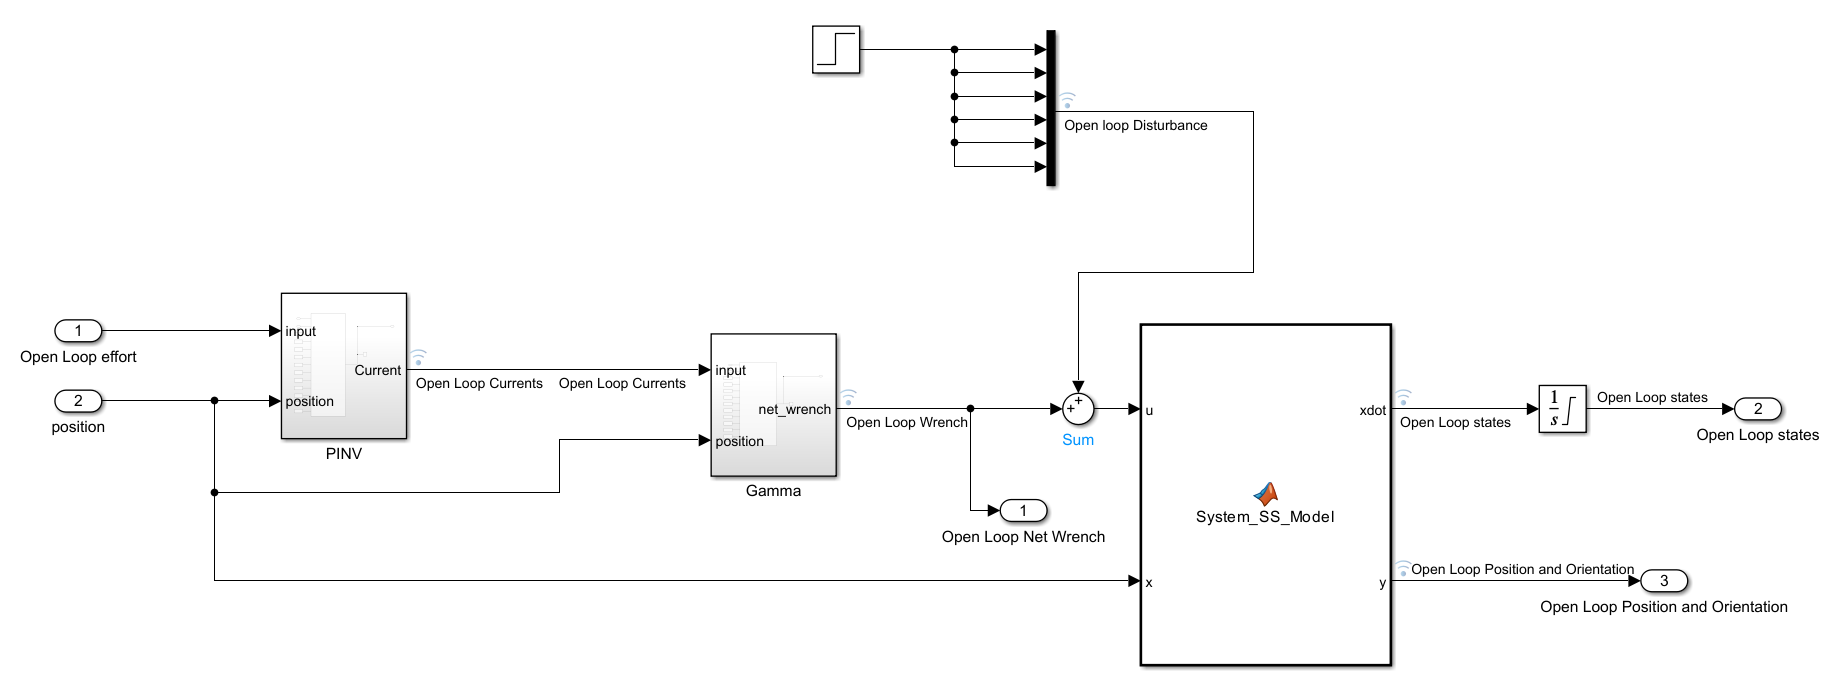
\includegraphics[width=1\linewidth]{../img/plant_Disturbance}
	\caption{دیاگرام سیستم با اغتشاش}
	\label{fig:plantdisturbance}
\end{figure}

با اعمال ورودی پله، پاسخ های حالت های سیستم به صورت زیر به دست می آیند.
\begin{figure}[H]
	\centering
	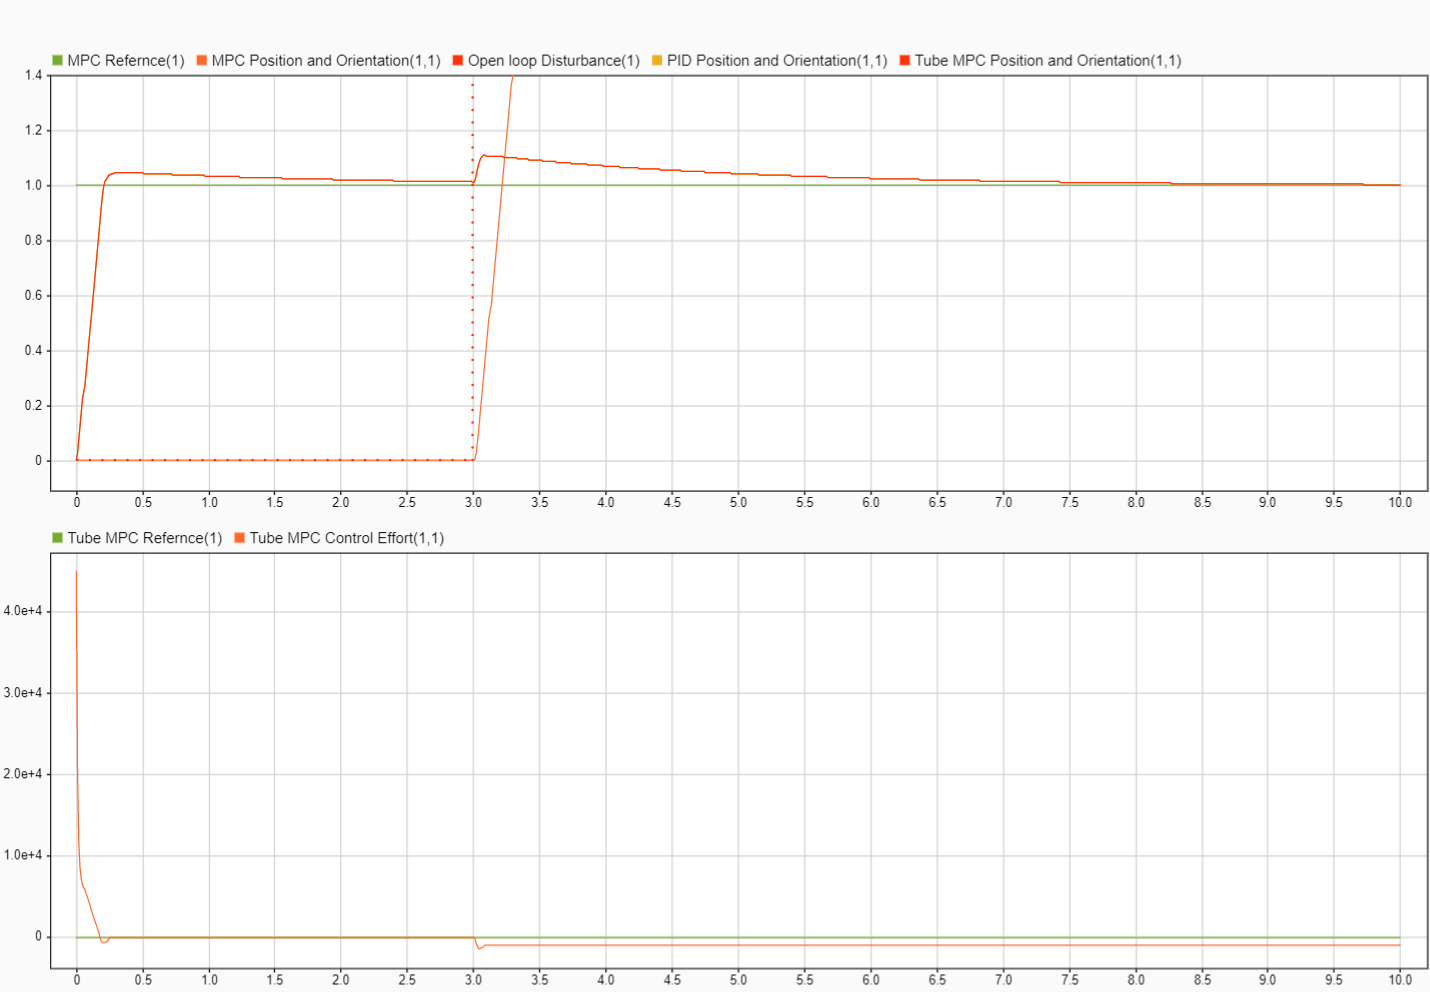
\includegraphics[width=1\linewidth]{../img/Disturbance_ResponseS1}
	\caption{پاسخ حالت اول به همراه اغتشاش}
	\label{fig:disturbanceresponses1}
\end{figure}
\begin{figure}[H]
	\centering
	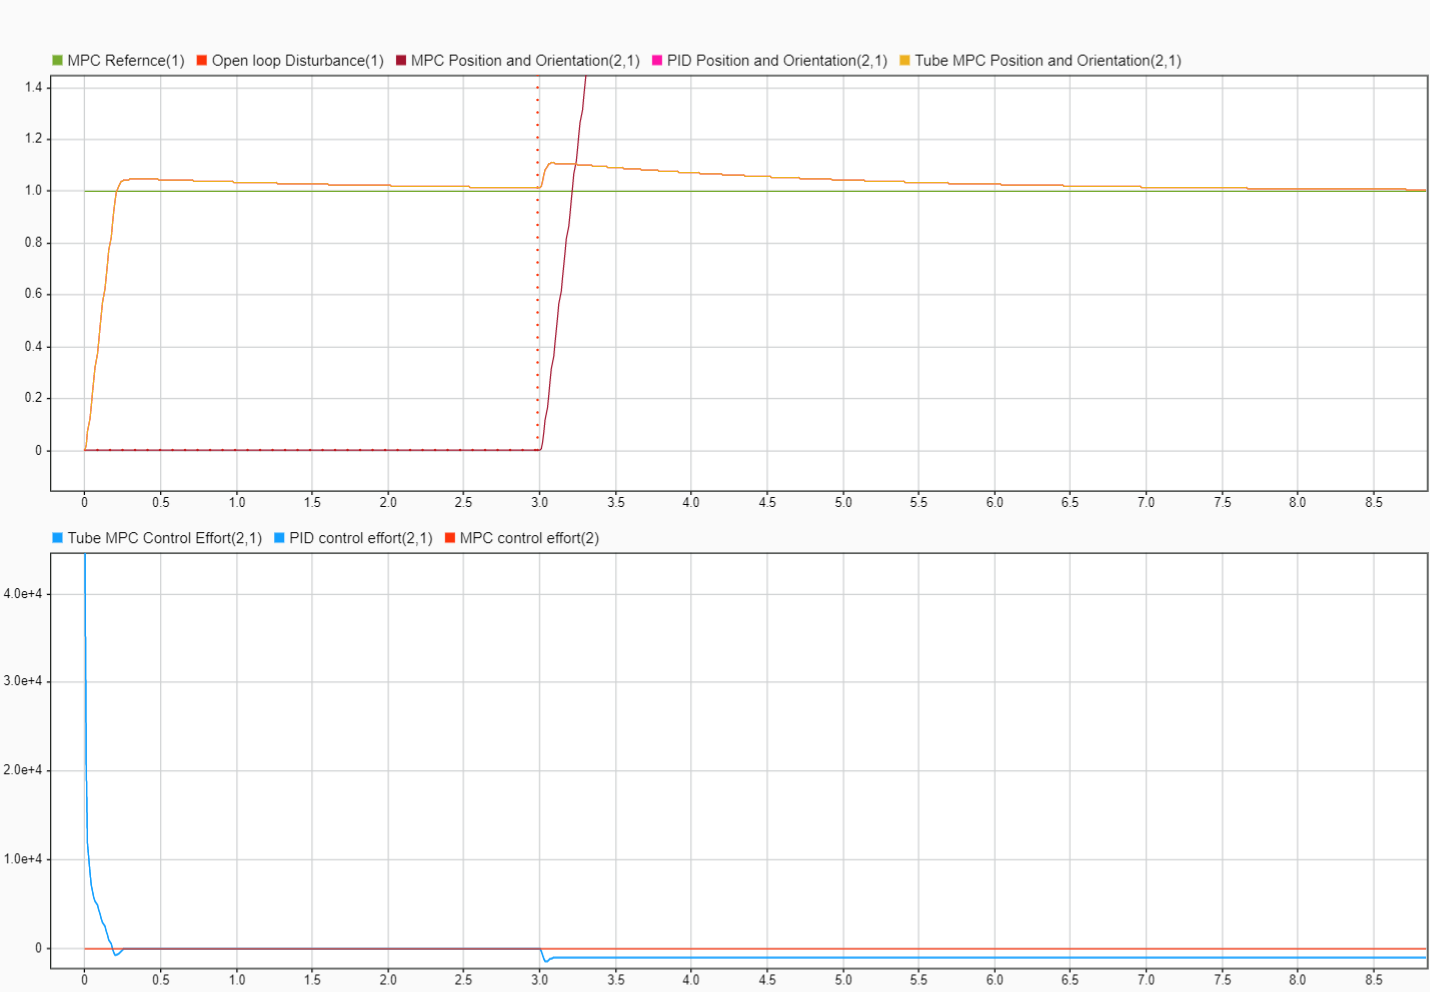
\includegraphics[width=1\linewidth]{../img/Disturbance_ResponseS2}
	\caption{پاسخ حالت دوم به همراه اغتشاش}
	\label{fig:disturbanceresponses2}
\end{figure}
\begin{figure}[H]
	\centering
	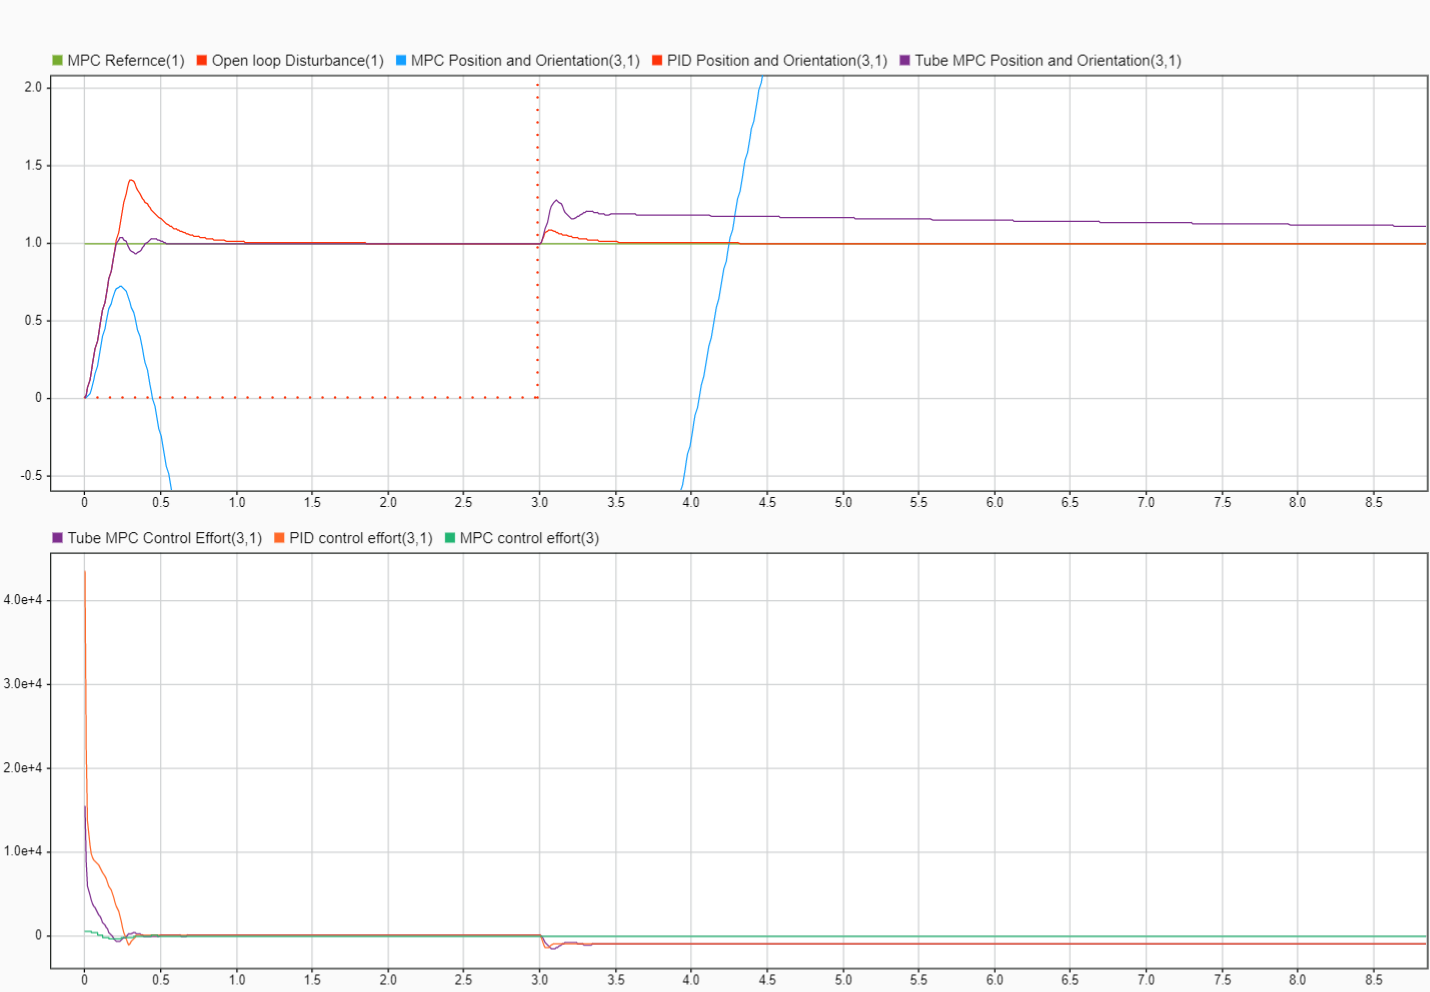
\includegraphics[width=1\linewidth]{../img/Disturbance_ResponseS3}
	\caption{پاسخ حالت سوم به همراه اغتشاش}
	\label{fig:disturbanceresponses3}
\end{figure}
\begin{figure}[H]
	\centering
	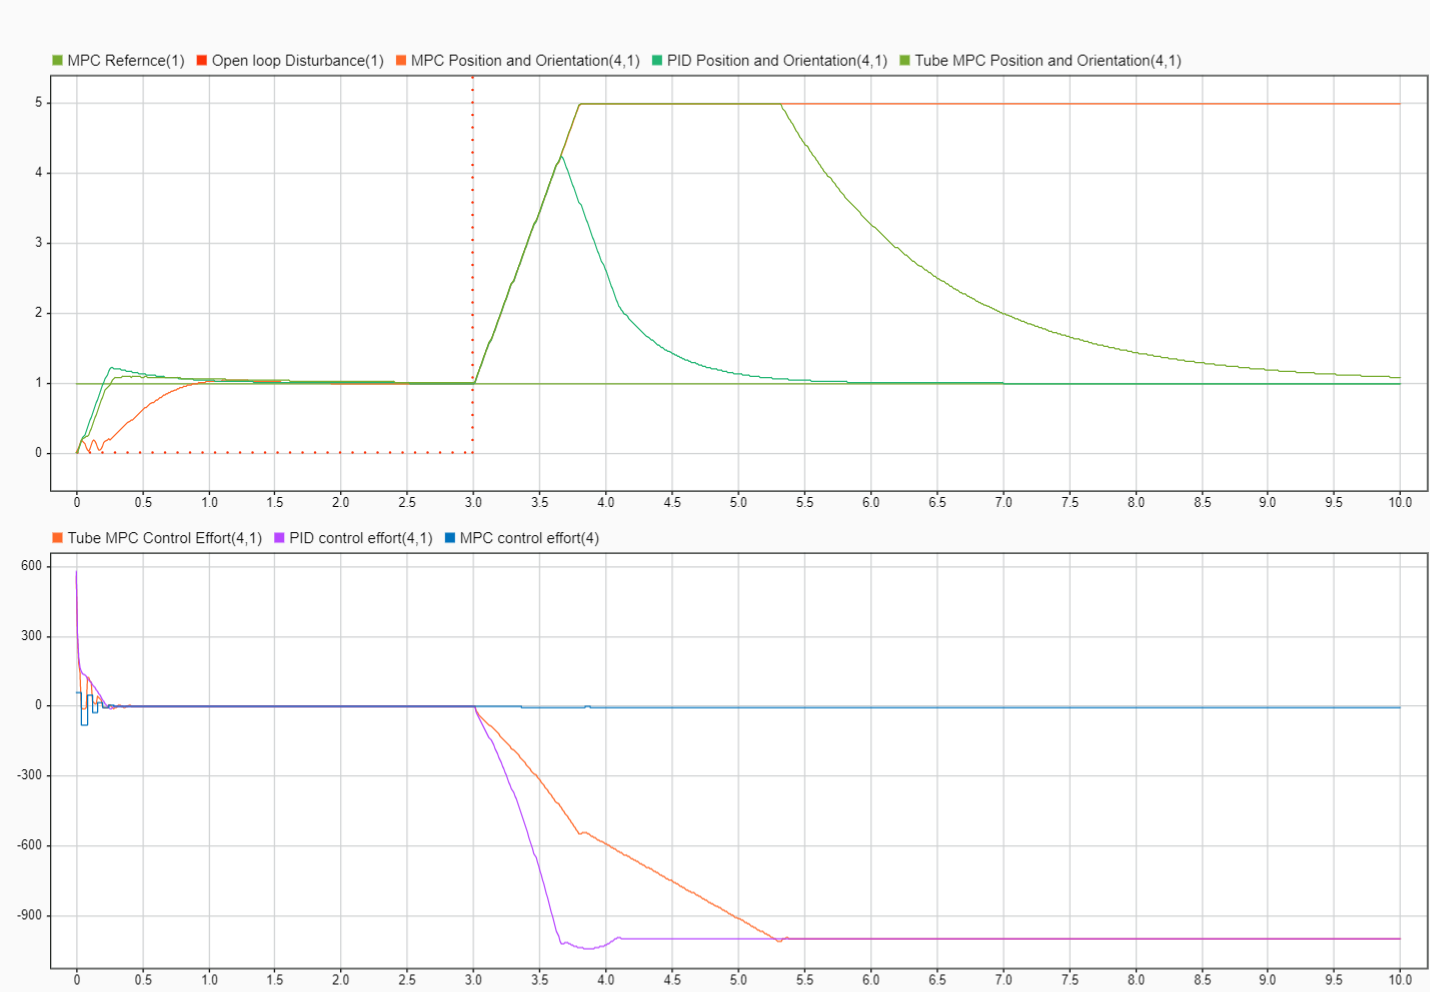
\includegraphics[width=1\linewidth]{../img/Disturbance_ResponseS4}
	\caption{پاسخ حالت چهارم به همراه اغتشاش}
	\label{fig:disturbanceresponses4}
\end{figure}
\begin{figure}
	\centering
	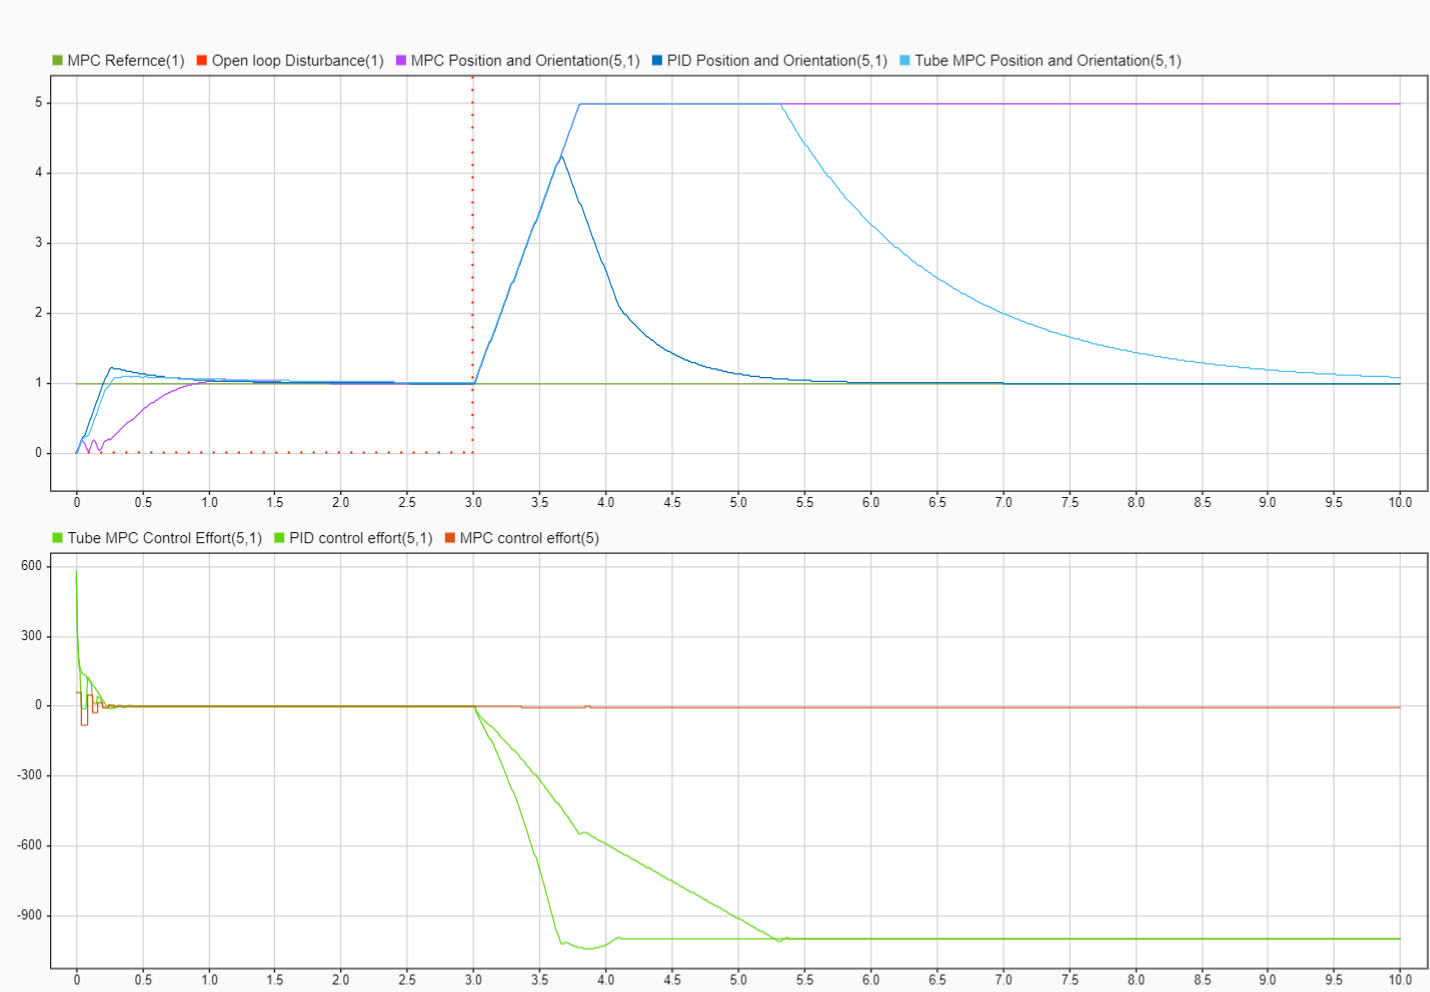
\includegraphics[width=1\linewidth]{../img/Disturbance_ResponseS5}
	\caption{پاسخ حالت پنجم به همراه اغتشاش}
	\label{fig:disturbanceresponses5}
\end{figure}
\begin{figure}[H]
	\centering
	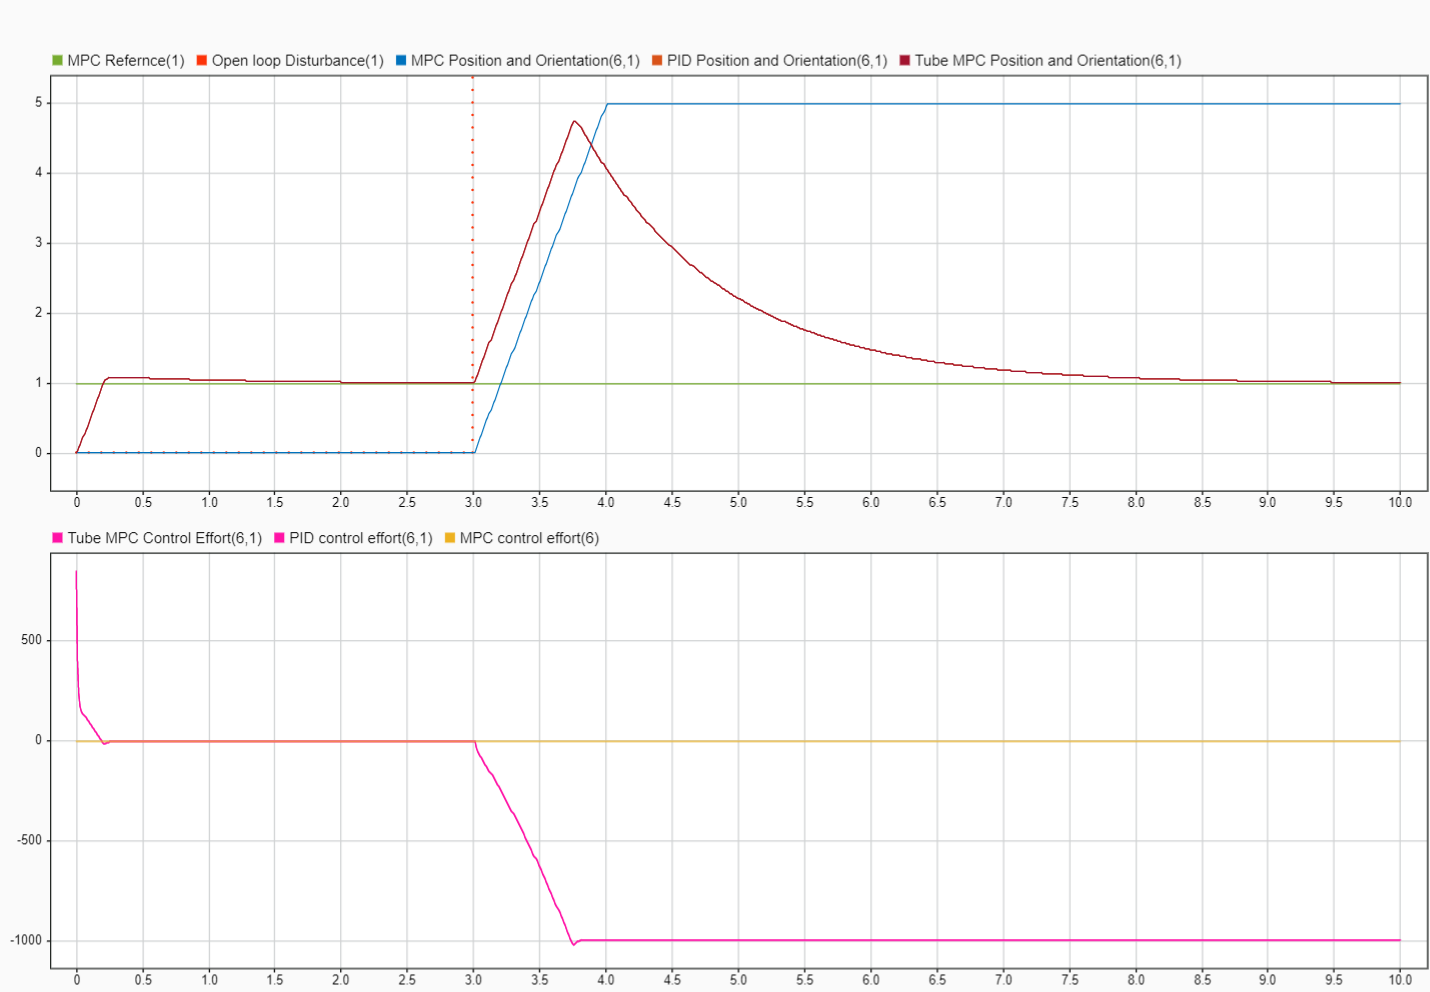
\includegraphics[width=1\linewidth]{../img/Disturbance_ResponseS6}
	\caption{پاسخ حالت ششم به همراه اغتشاش}
	\label{fig:disturbanceresponses6}
\end{figure}

